\documentclass{article}
\usepackage[utf8]{inputenc}
\usepackage{graphicx}

\title{Tugas 1 Pemrograman 2\\[1ex]}
\author{Oleh\\Alifia Zahra\\1184051\\D4 TI 2B\\\\\\\\POLITEKNIK POS INDONESIA\\BANDUNG\\2019}

\begin{document}

\maketitle

\newpage

\section{SEJARAH PYTHON}

        \paragraph{}Python pertama kali diciptakan oleh Guido van Rossum di  Centrum Wiskunde & Informatica (CWI) di Belanda pada awal tahun 1990-an. Pada tahun 1995, Guido melanjutkan pembuatan python di Corporation for National Research Initiative (CNRI) di Virginia Amerika, ia merilis beberapa versi dari python. 
        \par Pada tahun 2000 tepatnya di bulan Mei, Guido dan tim python pindah ke BeOpen.com lalu membentuk tim BeOpen PythonLabs. Lalu pada bulan Oktober, tim python pindah ke Digital Creation (sekarang menjadi Perusahaan Zope).
        \par Semua versi Python yang telah dirilis bersifat open source dan hampir semua menggunakan lisensi GFL-compatible. Adapun berbagai versi Python dan tanggal rilisnya sebagai berikut:
            \begin{enumerate}
            \item Python 1.0 – Januari 1994
            \item Python 1.2 – 10 April 1995
            \item Python 1.3 – 12 Oktober 1995
            \item Python 1.4 – 25 Oktober 1996
            \item Python 1.5 – 31 Desember 1997
            \item Python 1.6 – 5 September 2000
            \item Python 2.0 – 16 Oktober 2000
            \item Python 2.1 – 17 April 2001
            \item Python 2.2 – 21 Desember 2001
            \item Python 2.3 – 29 Juli 2003
            \item Python 2.4 – 30 Nopember 2004
            \item Python 2.5 – 19 September 2006
            \item Python 2.6 – 1 Oktober 2008
            \item Python 2.7 – 3 Juli 2010
            \item Python 3.0 – 3 Desember 2008
            \item Python 3.1 – 27 Juni 2009
            \item Python 3.2 – 20 Februari 2011
            \item Python 3.3 – 29 September 2012
            \item Python 3.4 – 16 Maret 2014
            \item Python 3.5 – 13 September 2015
            \item Python 3.6 – 23 Desember 2016
            \item Python 3.7 – 27 Juni 2018
            \end{enumerate}
        \par Perbedaan Python versi 2 dan 3 tidak jauh berbeda, python 2 dinilai lebih transparan dan inklusif untuk pengembangan software ketimbang versi sebelumnya. Python 2 dilengkapi dengan berbagai fitur programatikal seperti cycle-detecting garbage collector untuk mengotomasi manajemen memori, peningkatan dukungan untuk Unicode, list comprehension untuk membuat sebuah list dari list yang sudah ada. Python 3 sendiri adalah versi dengan banyak perubahan yang dirilis pada akhir tahun 2008. Fokus dari Python 3 itu sendiri adalah untuk melakukan perapian pada codebase dan menghapuskan duplikasi (redundancy). Perubahan terbesar pada Python 3 termasuk memasukkan statemen print ke dalam built-in function. Contoh perbedaan pertama terletak dalam pemakaian syntax, pada Python 2 kita bisa menggunakan tanda kurung atau tidak, sedangkan di Python 3 wajib jika tidak hasilnya akan error. 
        
\subsection{Implementasi dan Penggunaan Python pada Perusahaan}
    \begin{enumerate}
        \item Instagram menggunakan Django, framework python sebagai mesin pengolah sisi server dari aplikasinya.
        \item Tim Spotify memanfaatkan analitis, memanfaatkan Luigi, modul dari Python, yang disinkronisasi dengan Hadoop, sebuah framework berbasis Java yang memungkinkan pemrosesan data dengan ukuran sangat besar.
        \item Penggunaan utama Python pada Netflix adalah pada Central Alert Gateway. Ini akan me-reroute alert dan mengirimkan pada individu/kelompok yang ingin melihat. Selain itu Python digunakan pada aplikasi untuk menelusuri riwayat dan perubahan pengaturan keamanan.
    \par Dan masih banyak perusahaan besar yang menggunakan Python
    \end{enumerate}    
    
\newpage    
\section{INSTALASI}
\subsection{Instalasi Python 3}
\begin{enumerate}
    \item Pertama download Anaconda sesuai OS yang anda pakai, anda dapat mengunduhnya di https://www.python.org/downloads/release/python-370.
    \item Setelah terunduh, klik dua kali pada file instalasi tersebut. Lalu akan muncul tampilan seperti ini, klik next.
        \begin{figure}[h]
            \centerline{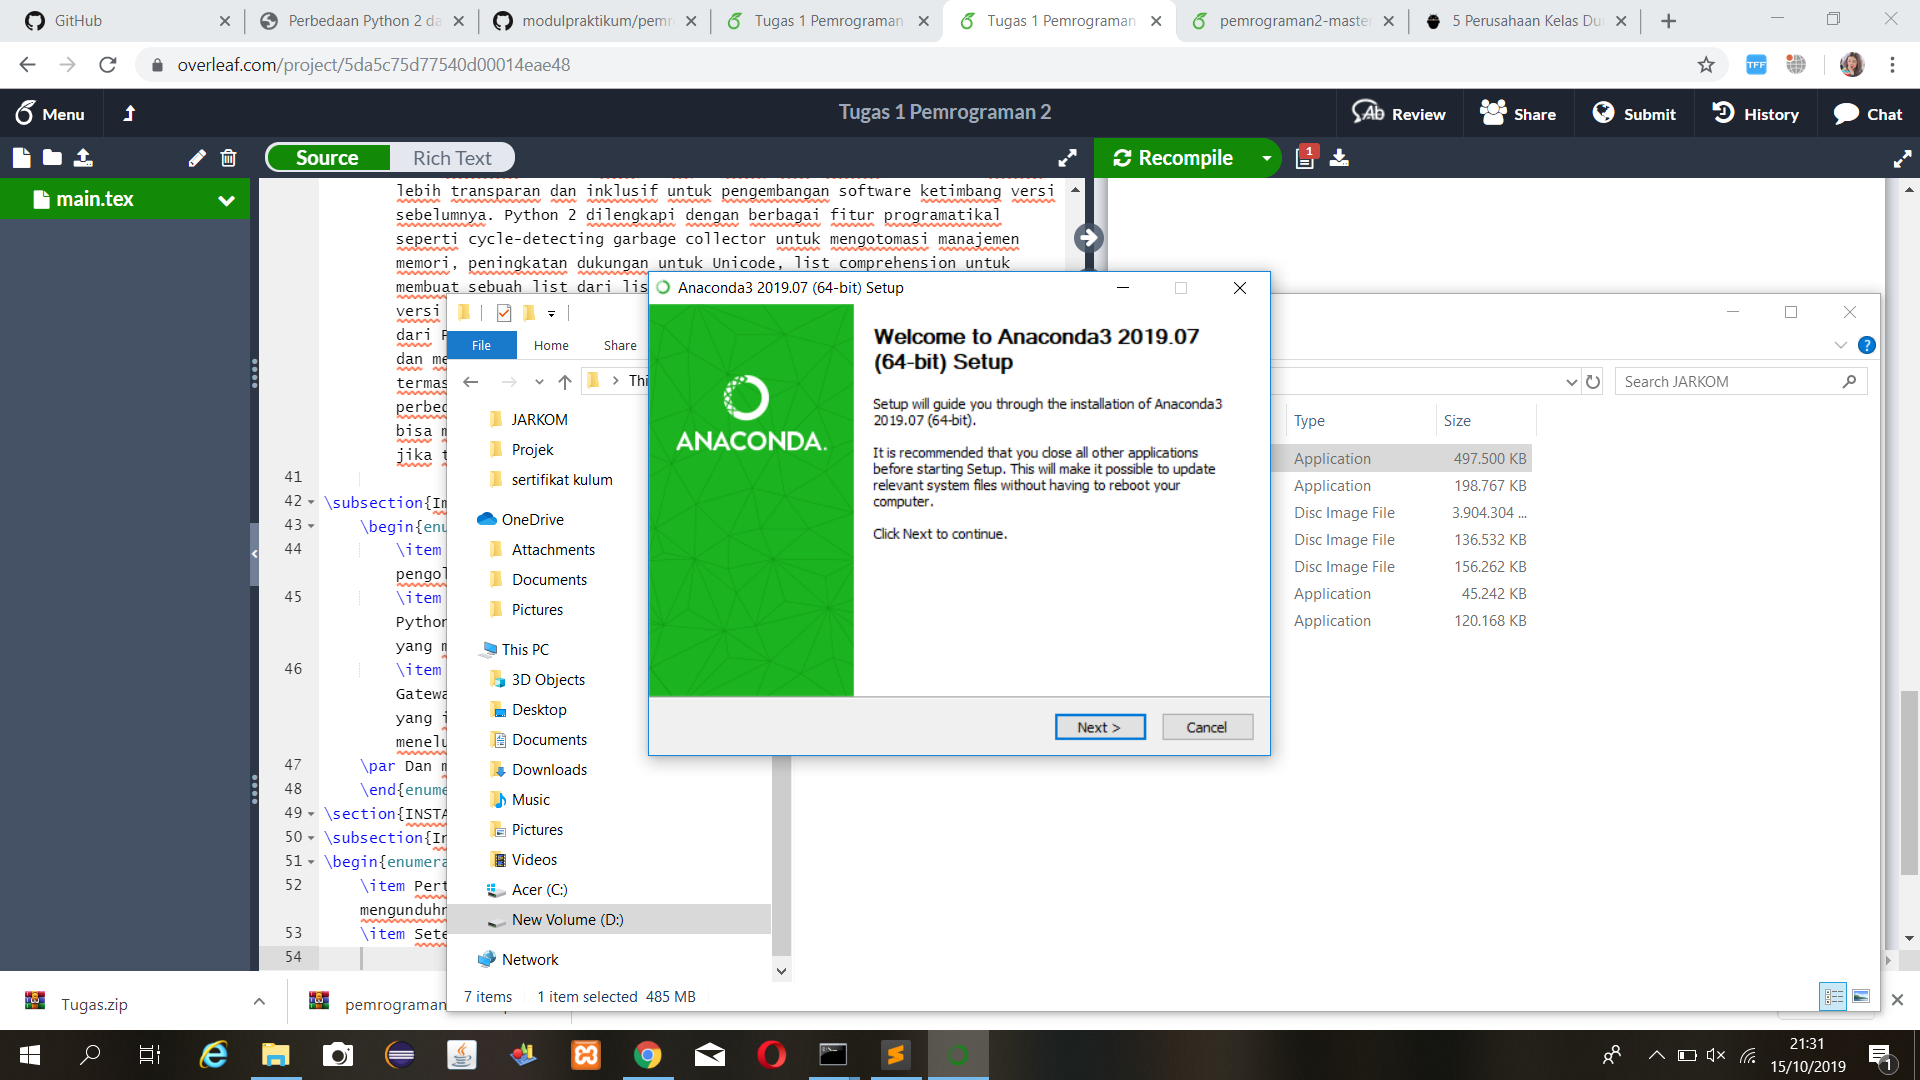
\includegraphics[width=8cm]{image/langkah1.png}}
        \end{figure}
    \item Klik I agree, untuk menyetujui license instalasi Anaconda.
        \begin{figure}[h]
            \centerline{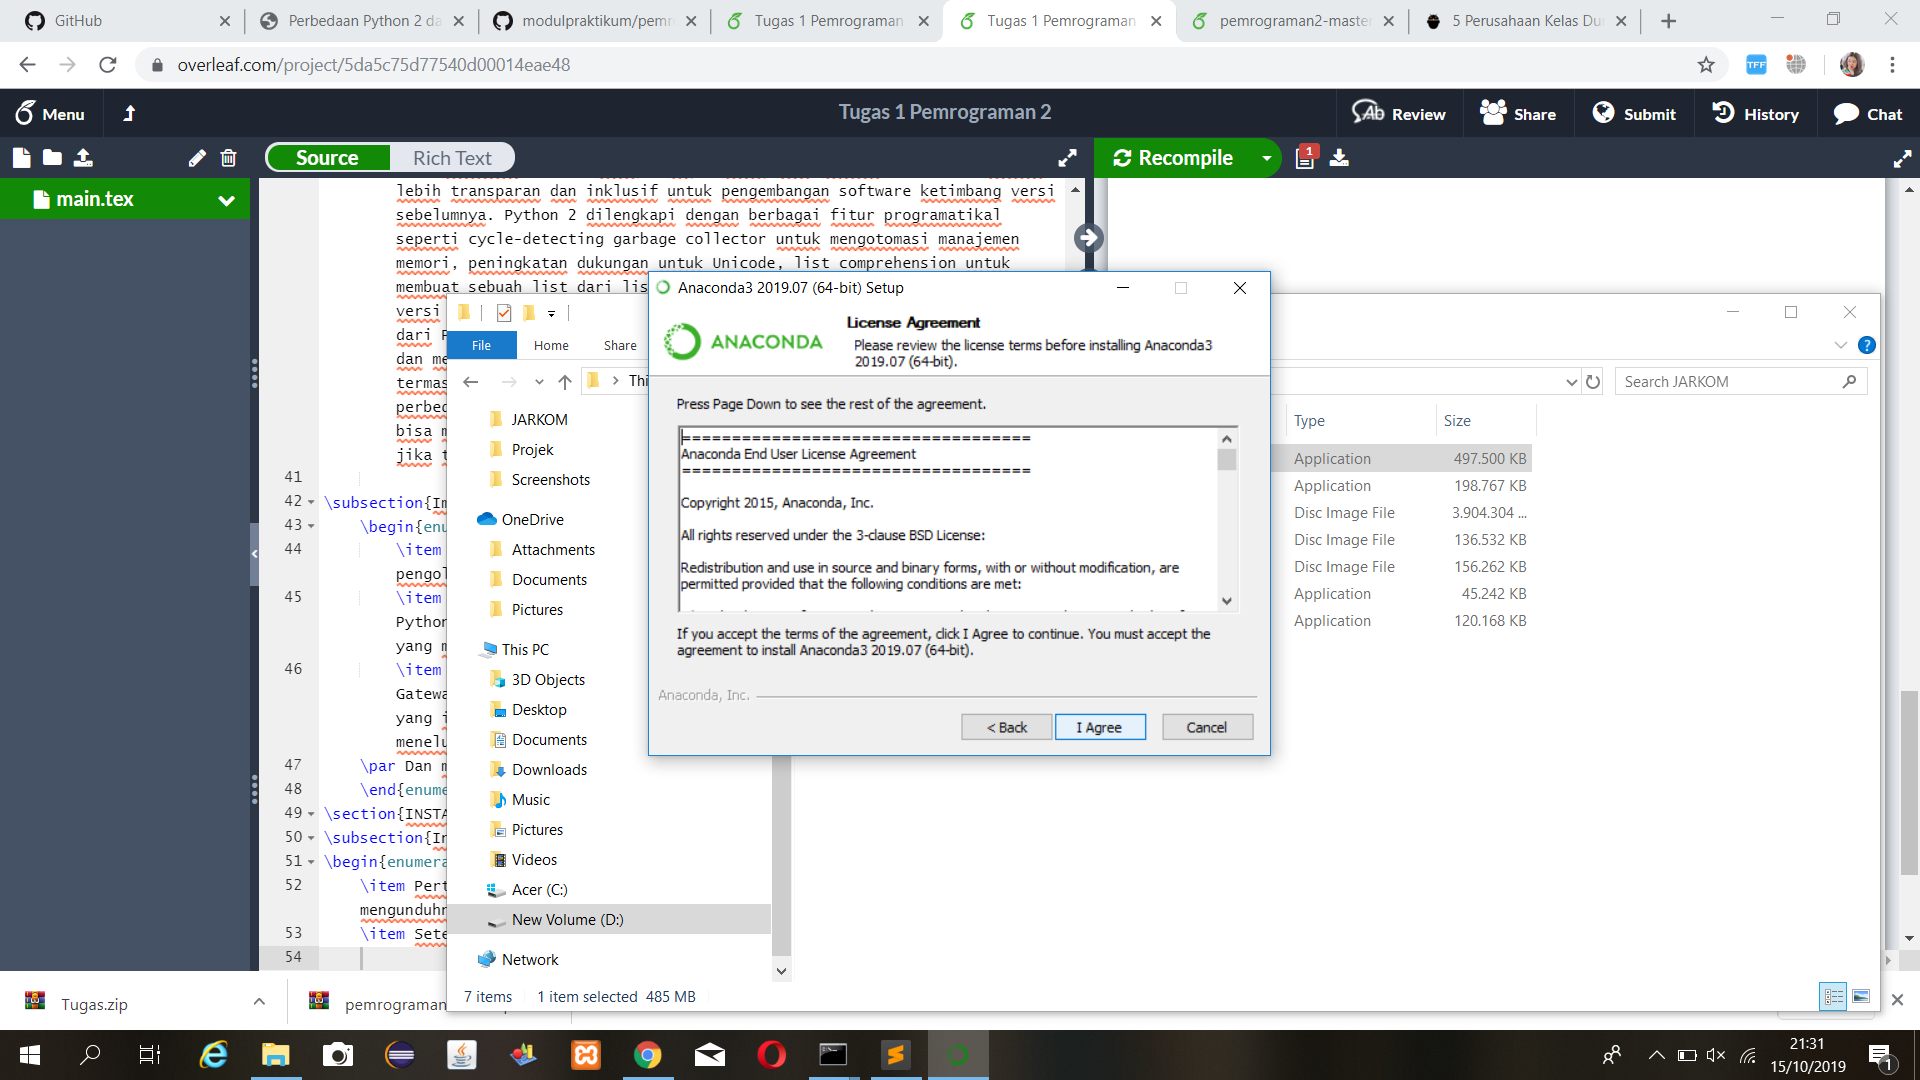
\includegraphics[width=8cm]{image/langkah2.png}}
        \end{figure}
    \item Lalu pilih installation tipe, klik just me (yg direkomendasikan).
        \paragraph{}
            \centerline{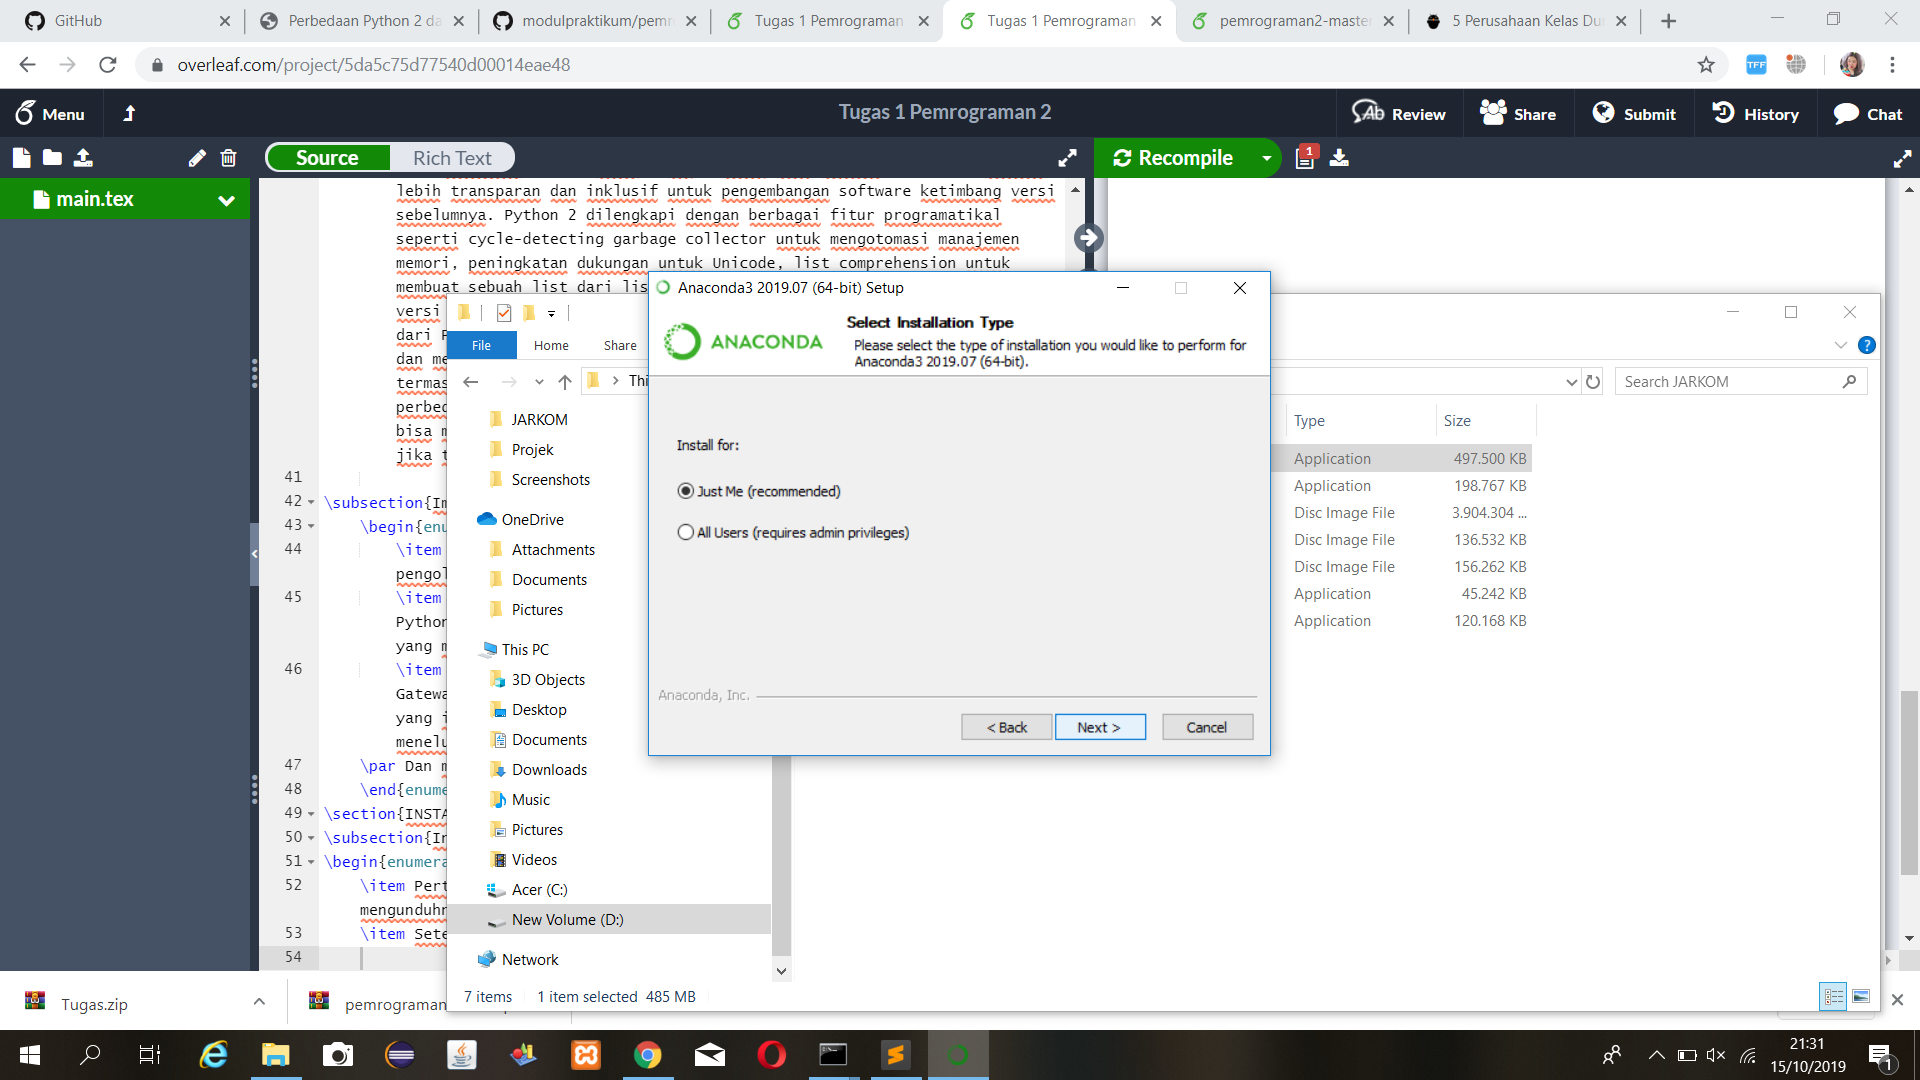
\includegraphics[width=8cm]{image/langkah3.png}}
    \item Lalu pilih tempat atau lokasi direktori untuk instalasi Anaconda, klik next.
        \begin{figure}[h]
            \centerline{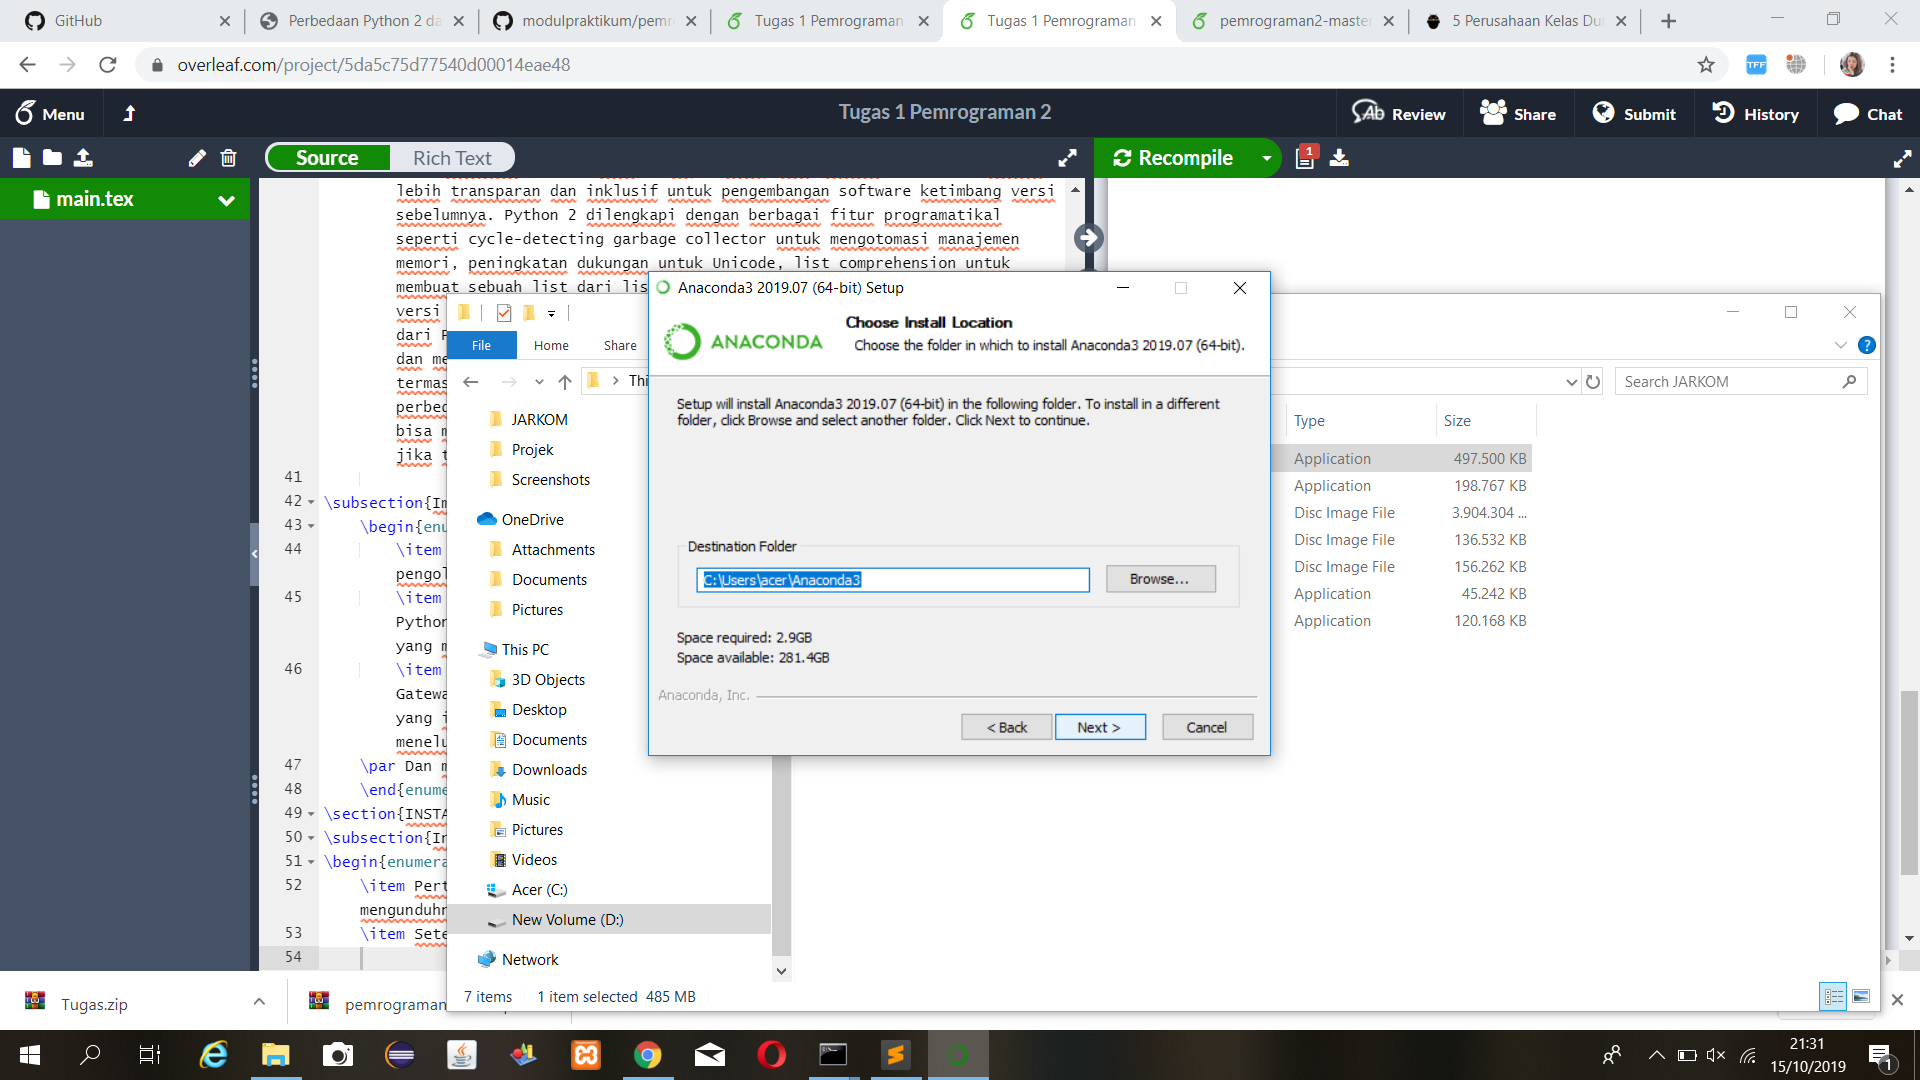
\includegraphics[width=8cm]{image/langkah4.png}}
        \end{figure}
    \item Untuk advance option, pilih dua opsi tersebut. Tunggu hingga instalasi Anaconda selesai.
        \begin{figure}[h]
            \centerline{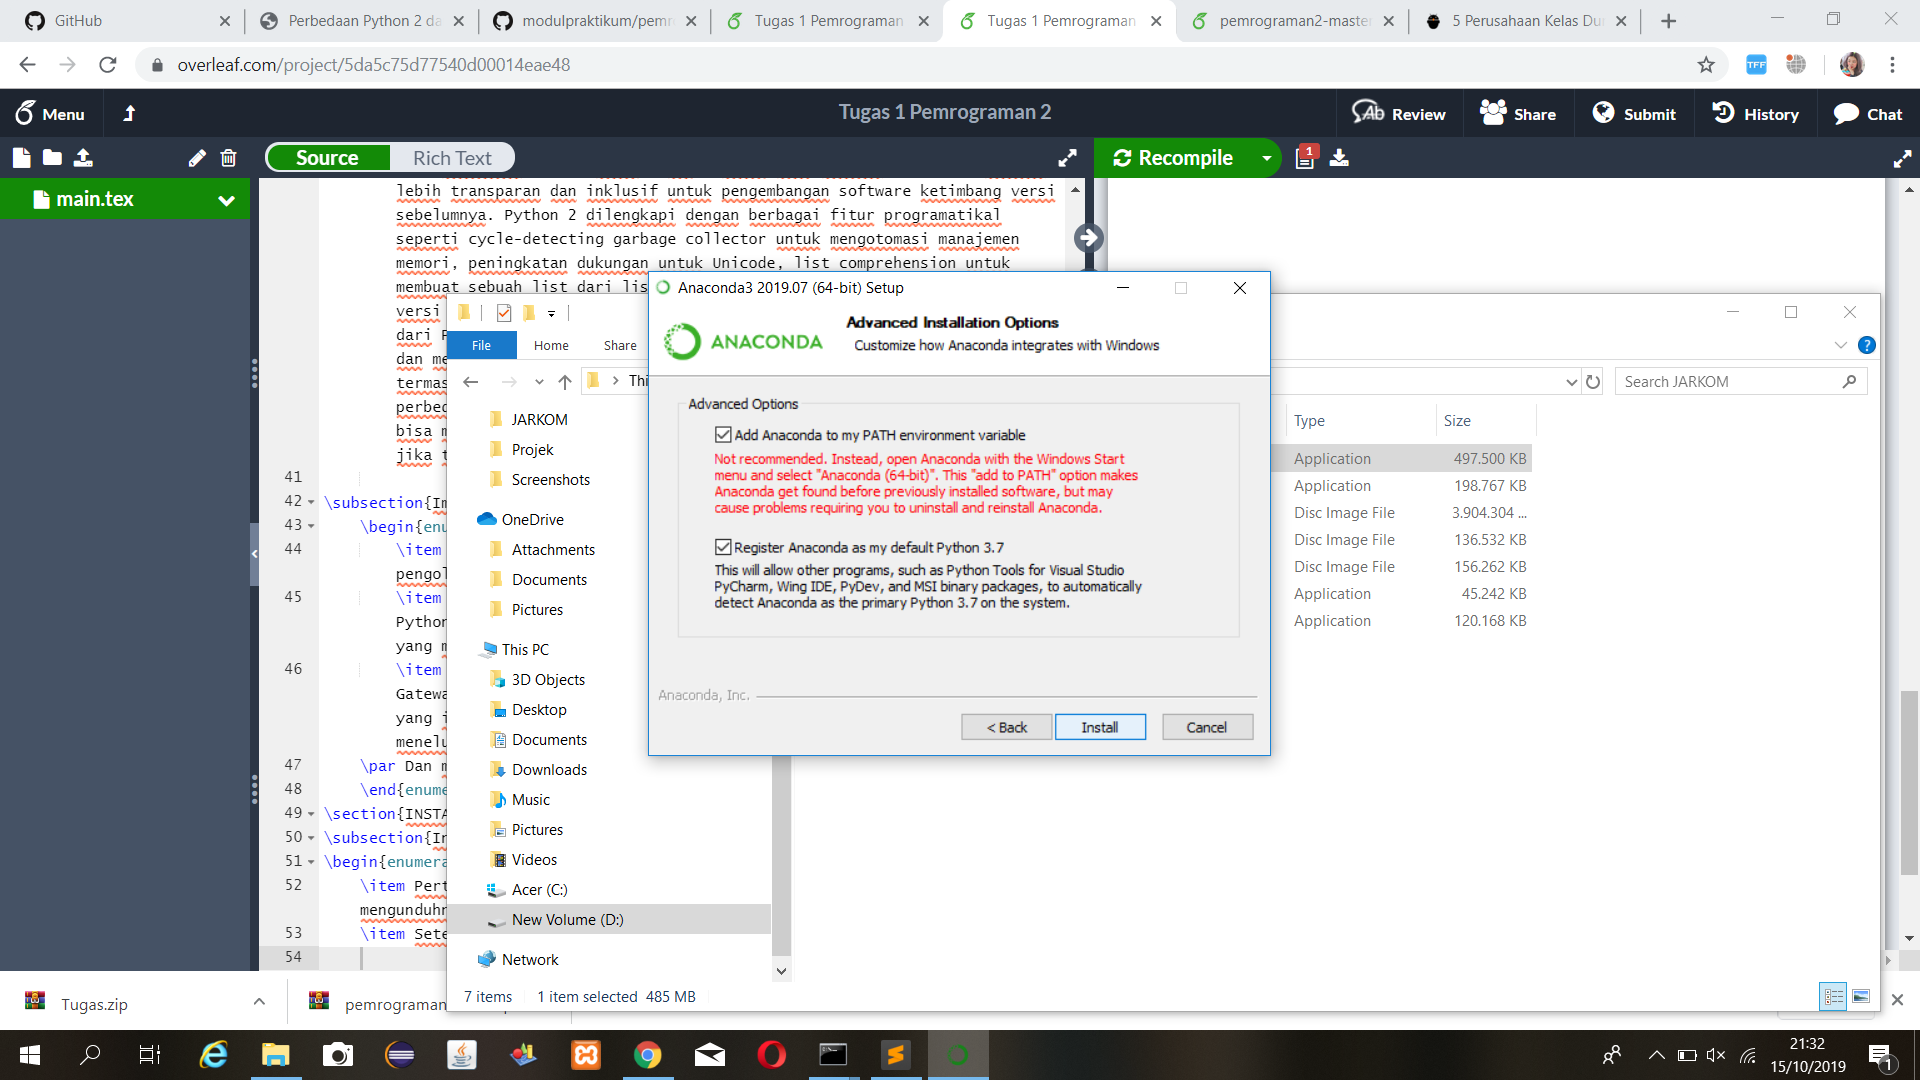
\includegraphics[width=8cm]{image/langkah5.png}}
        \end{figure}
\end{enumerate}

\newpage
\subsection{Instalasi PIP}
\begin{enumerate}
    \item Pertama buka Anaconda promt atau dengan meng-klik tombol jendela windows dan huruf R secara bersamaan, maka akan menampilkan gambar seperti di bawah. Pilih cmd kemudian tekan OK.
        \begin{figure}[h]
            \centerline{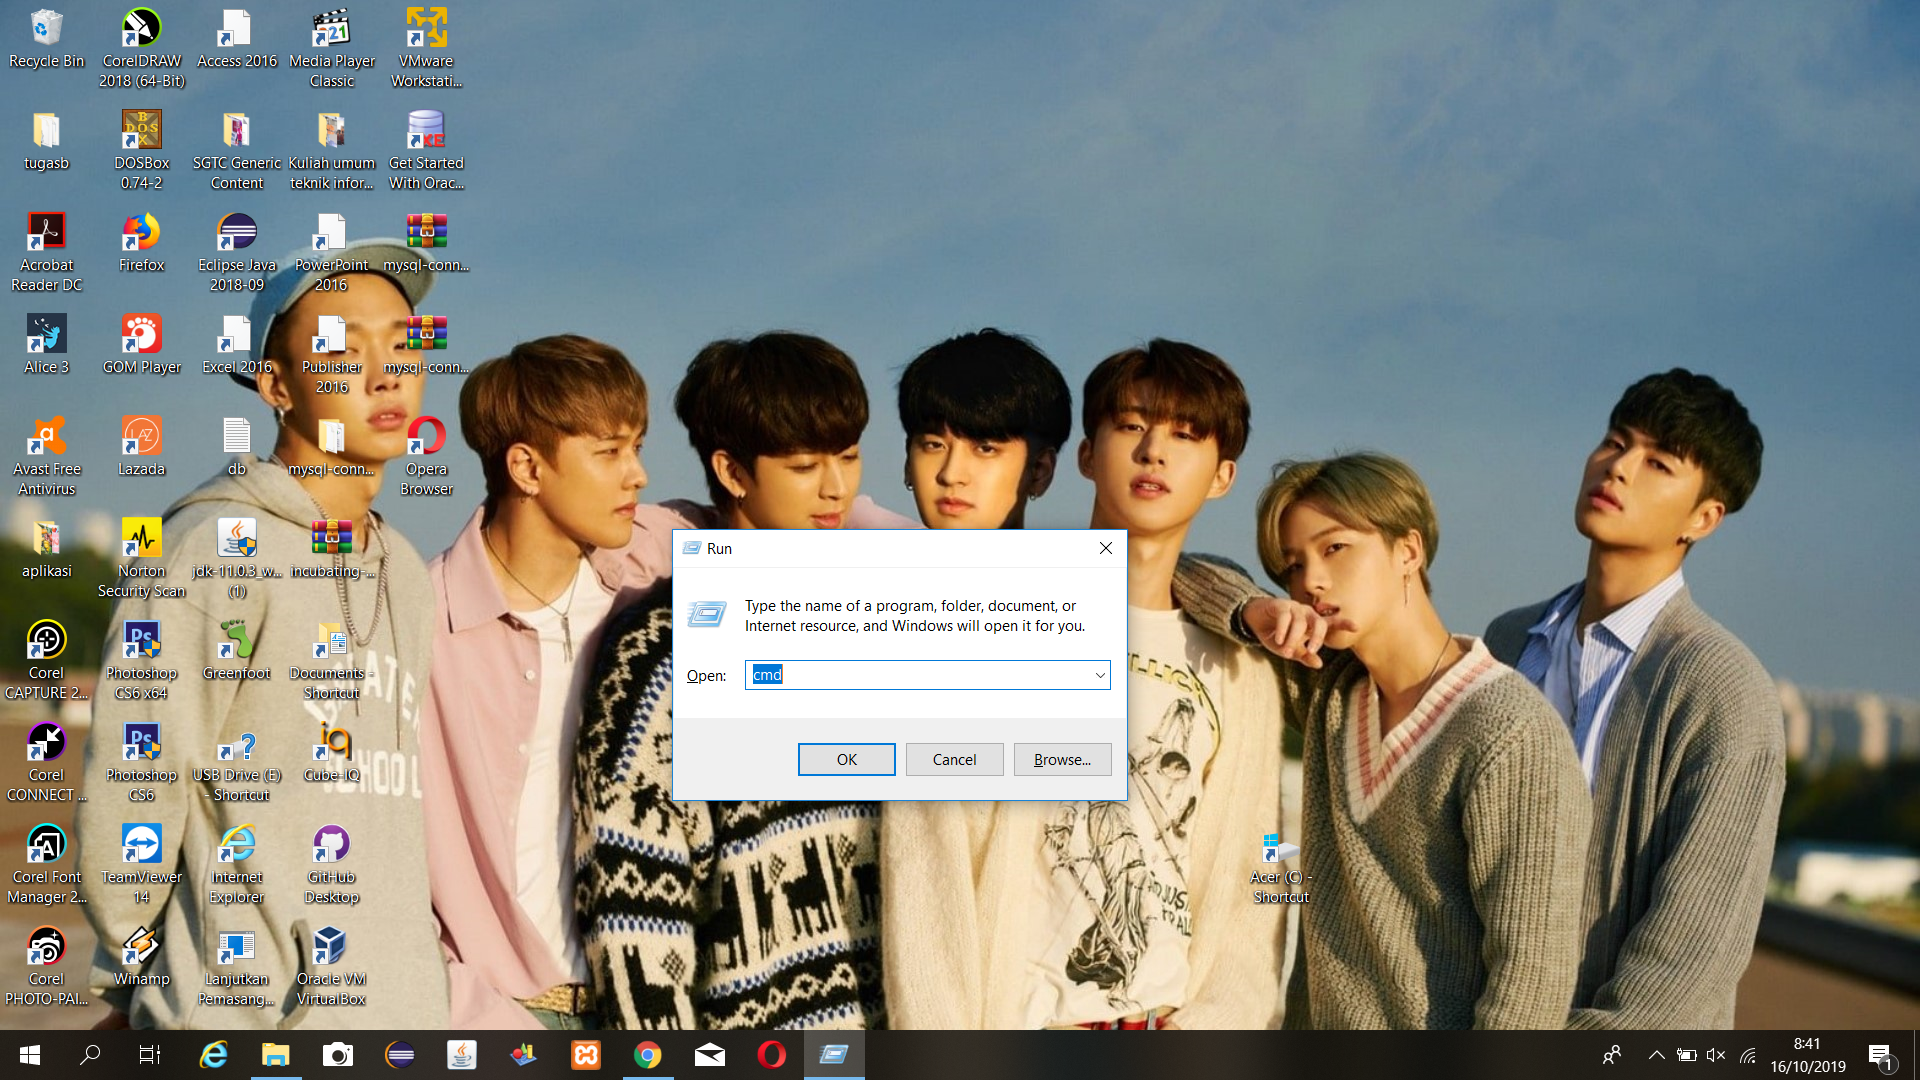
\includegraphics[width=8cm]{image/cmd.png}}
        \end{figure}
    \item Lalu ketikkan pip install requests.
        \begin{figure}[h]
            \centerline{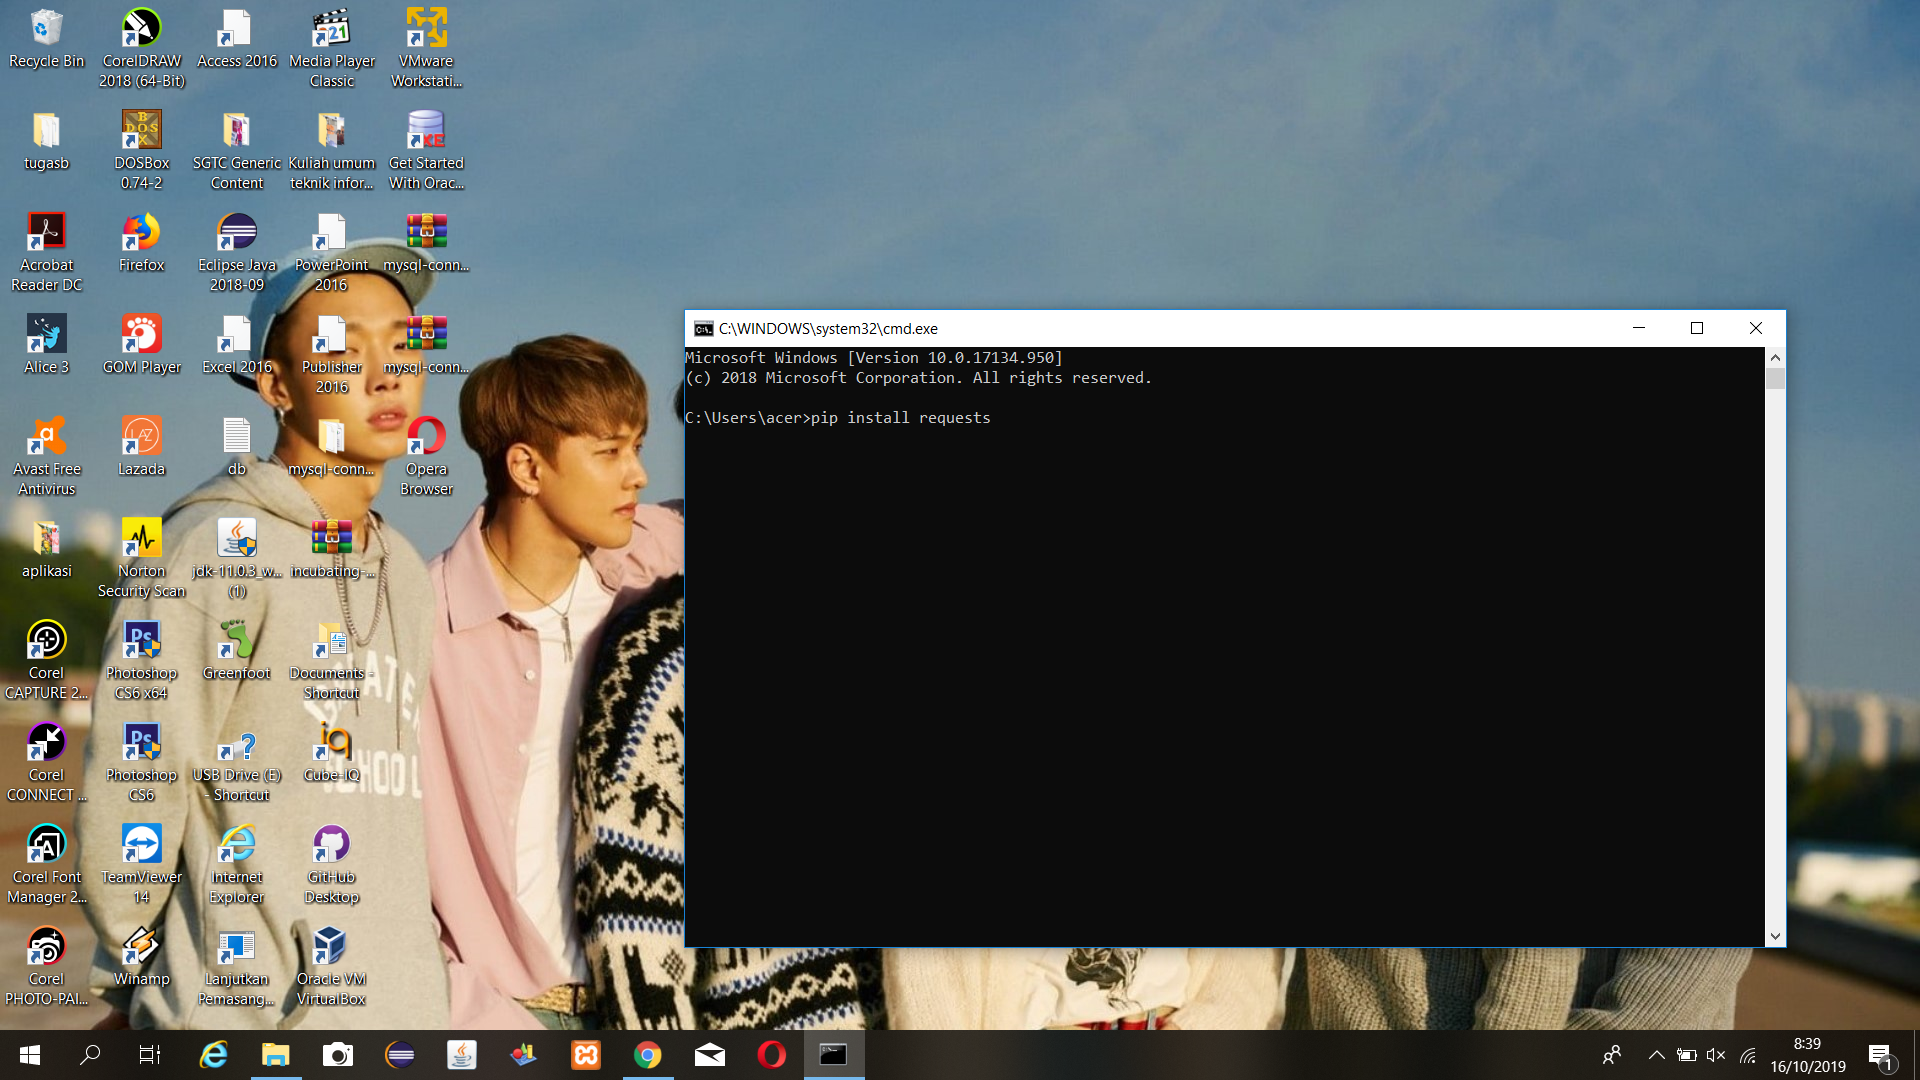
\includegraphics[width=8cm]{image/pip.png}}
        \end{figure}
    \item Jika berhasil maka akan keluar seperti berikut, jika gagal maka akan muncul pesan error.
            \paragraph{}
            \centerline{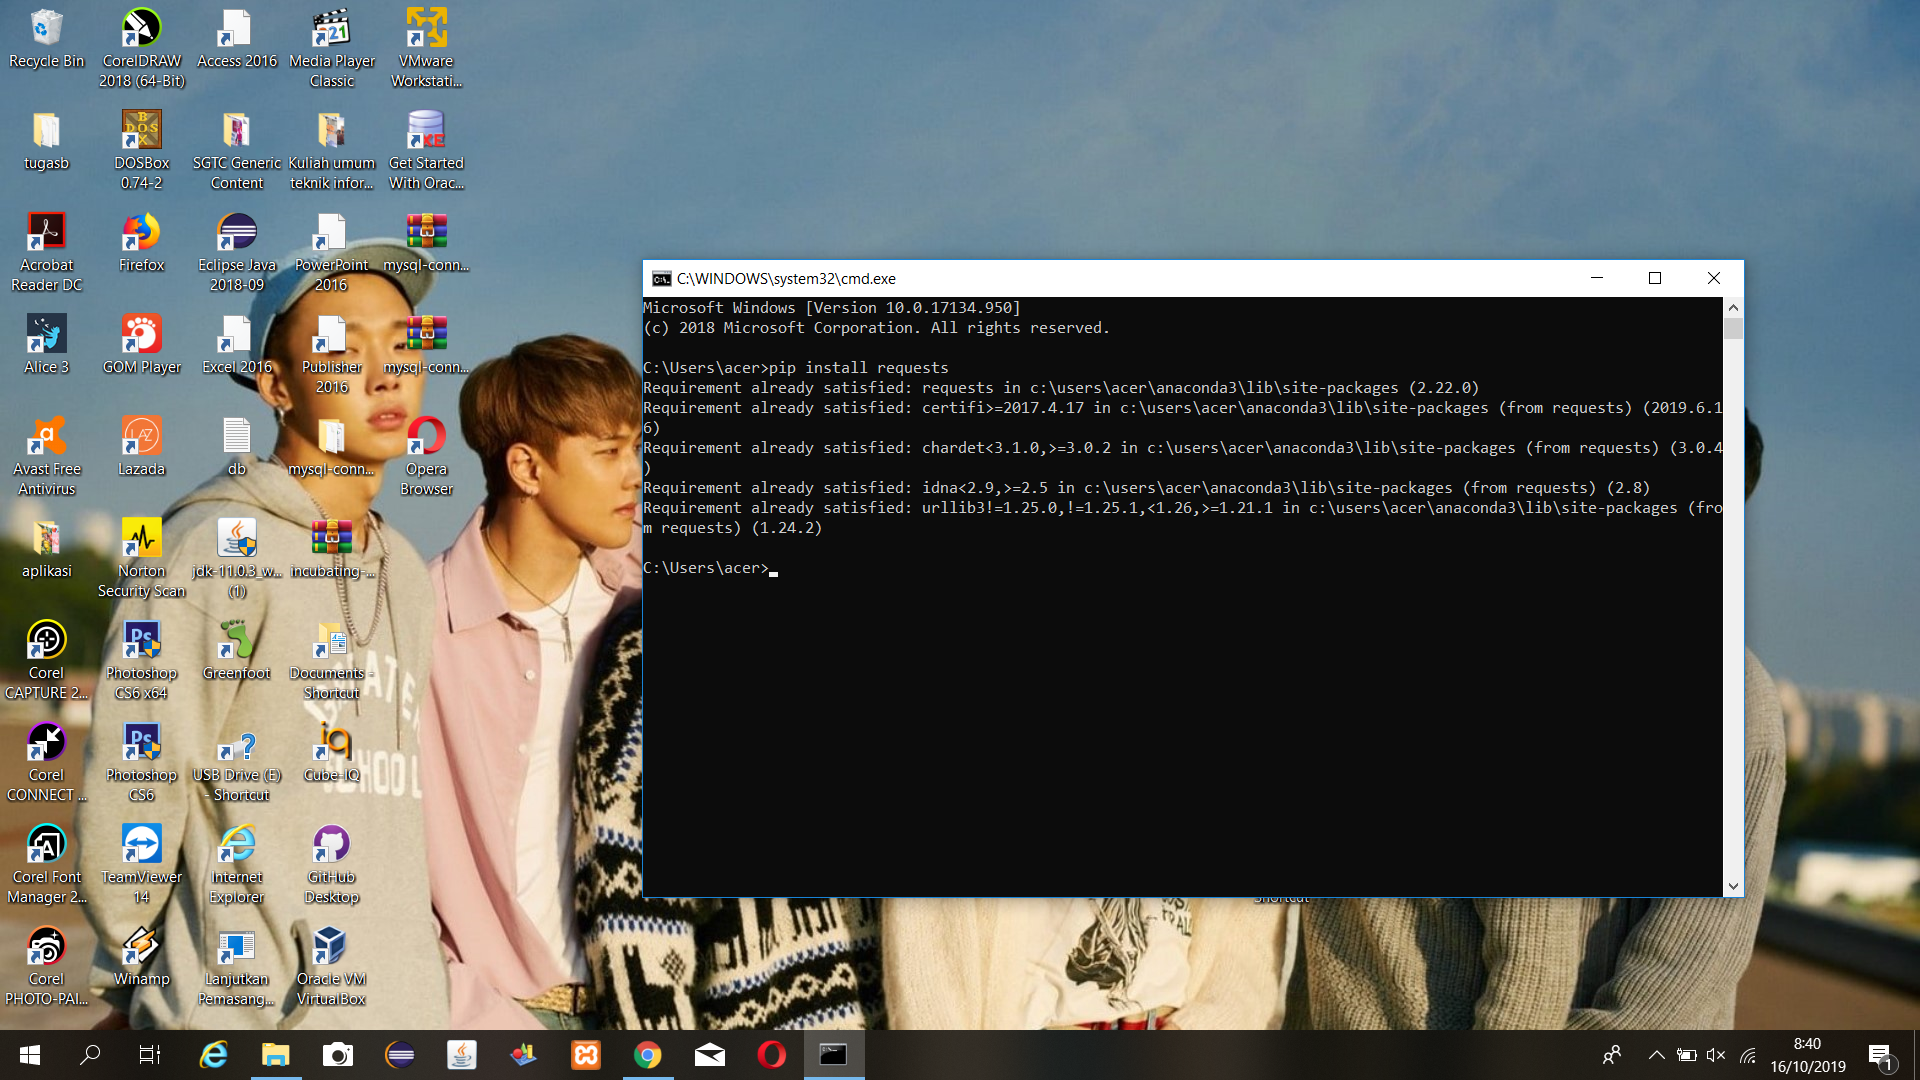
\includegraphics[width=8cm]{image/pipberhasil.png}}
\end{enumerate}

\subsection{Setting Environment}
\begin{enumerate}
    \item Pertama masuk ke control panel lalu pilih system dan security
        \begin{figure}[h]
            \centerline{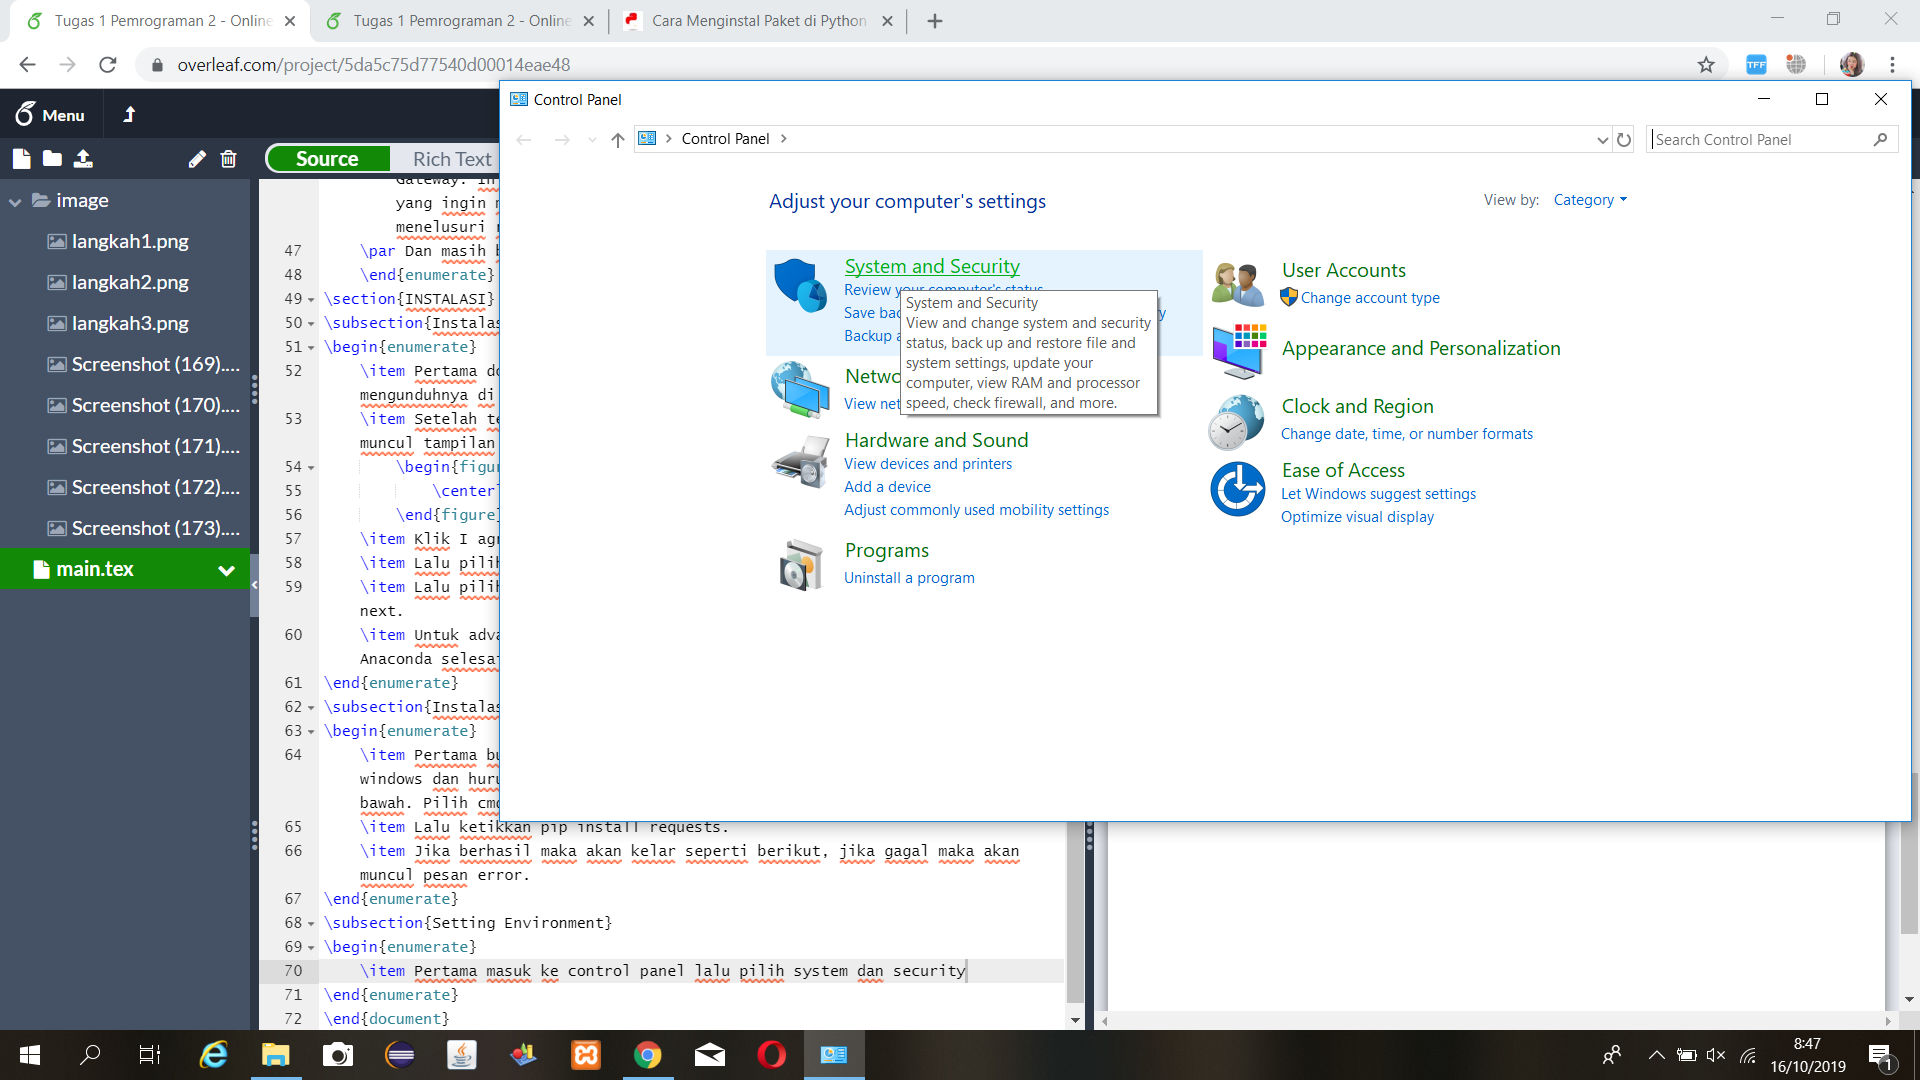
\includegraphics[width=8cm]{image/cpanel.png}}
        \end{figure}
    \item Lalu pilih Security and Maintanance
        \begin{figure}[h]
            \centerline{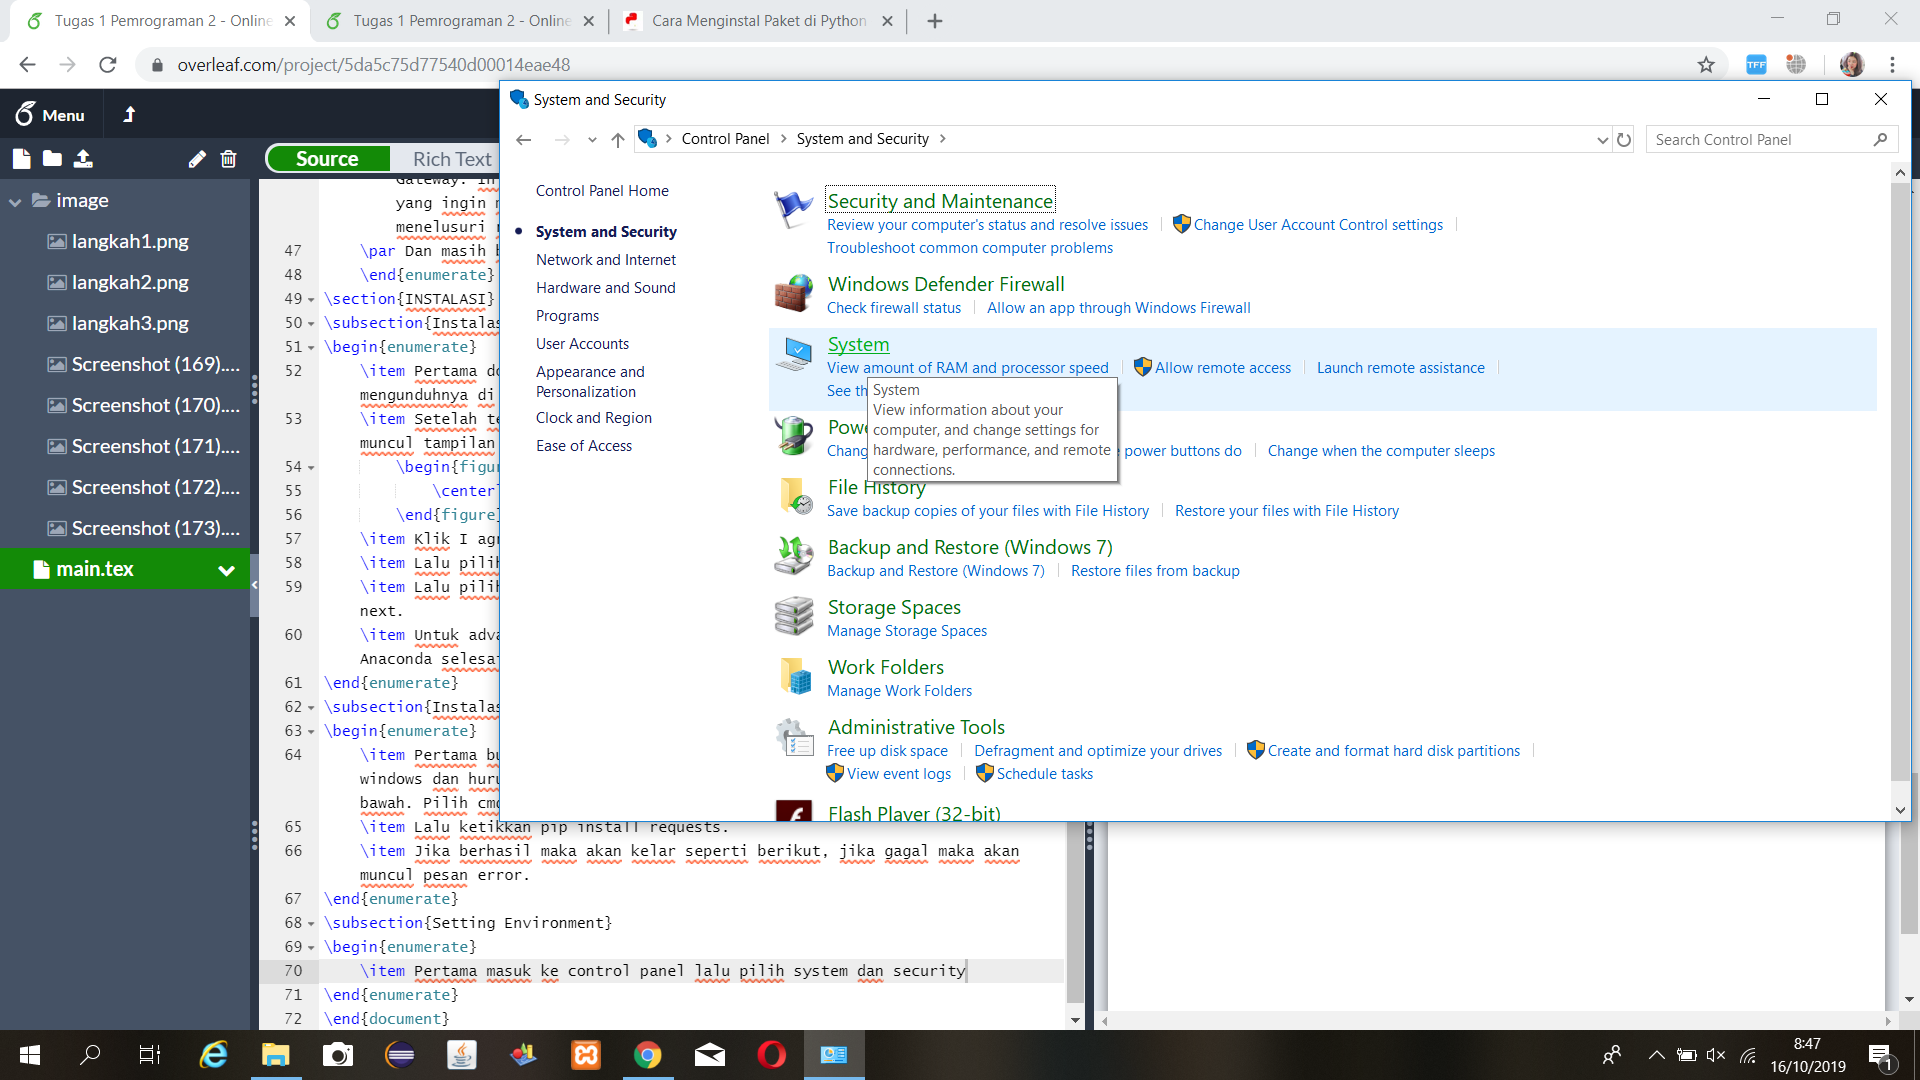
\includegraphics[width=8cm]{image/securityandmain.png}}
        \end{figure}
    \item Lalu pilih System dan Advanced System Settings.
            \paragraph{}
            \centerline{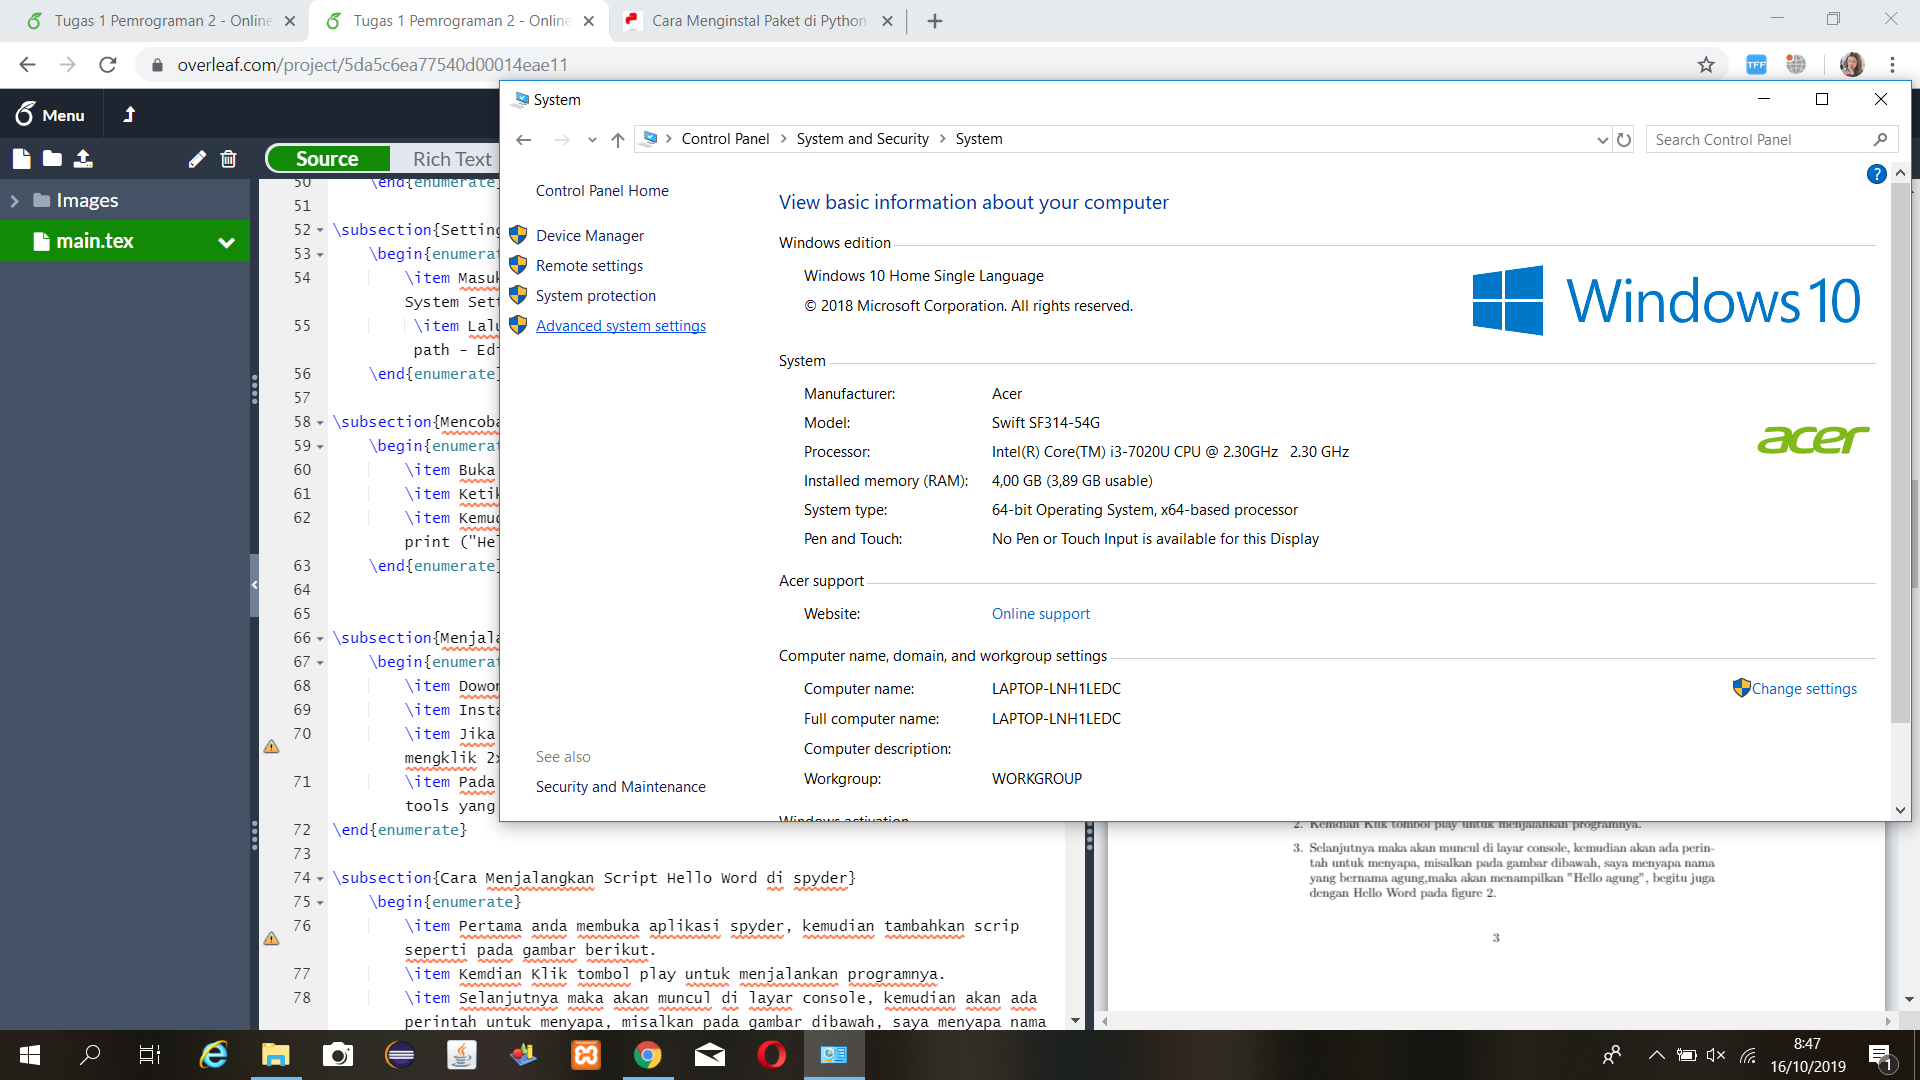
\includegraphics[width=8cm]{image/advanced.png}}
    \item Lalu pilih environment variables, lalu di System Variables klik path-Edit-New-C:/Python3/Scripts lalu klik OK.
        \begin{figure}[h]
            \centerline{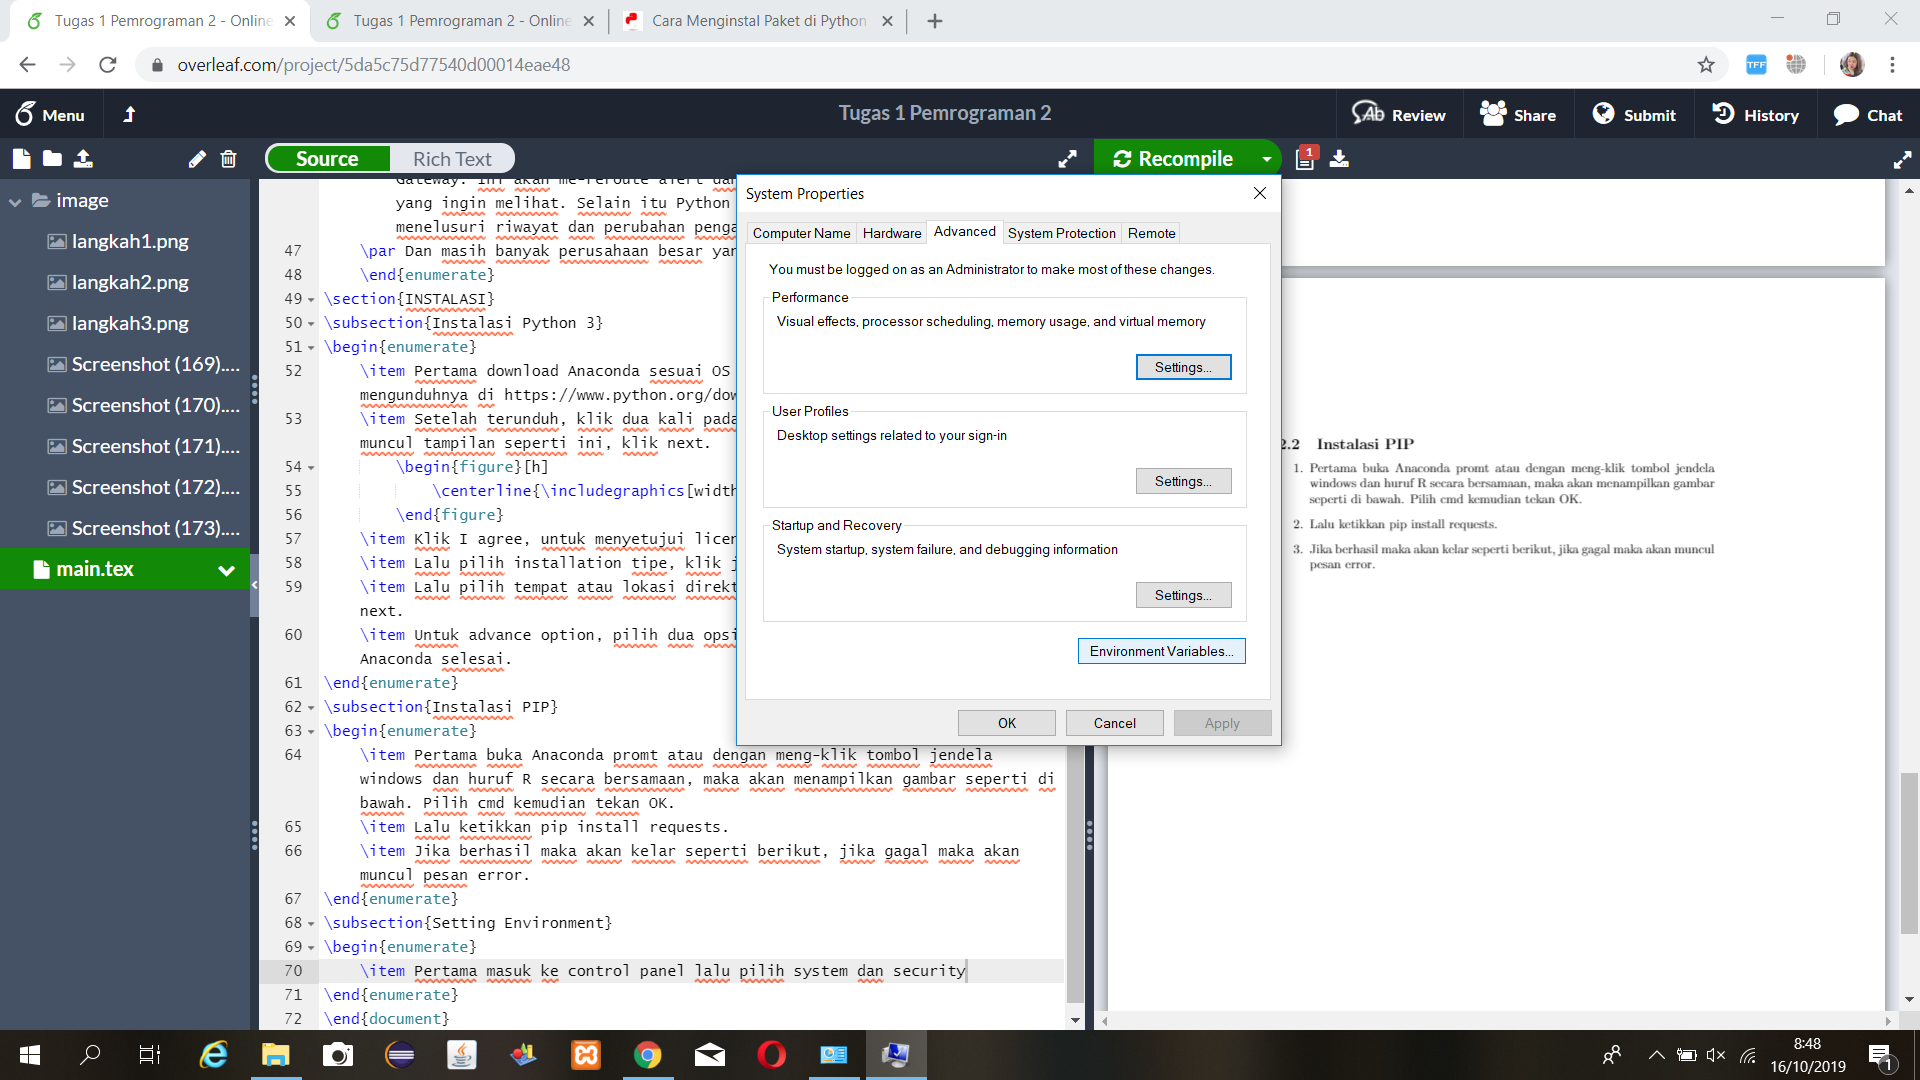
\includegraphics[width=8cm]{image/environtmentvar.png}}
        \end{figure}
        \begin{figure}[h]
            \centerline{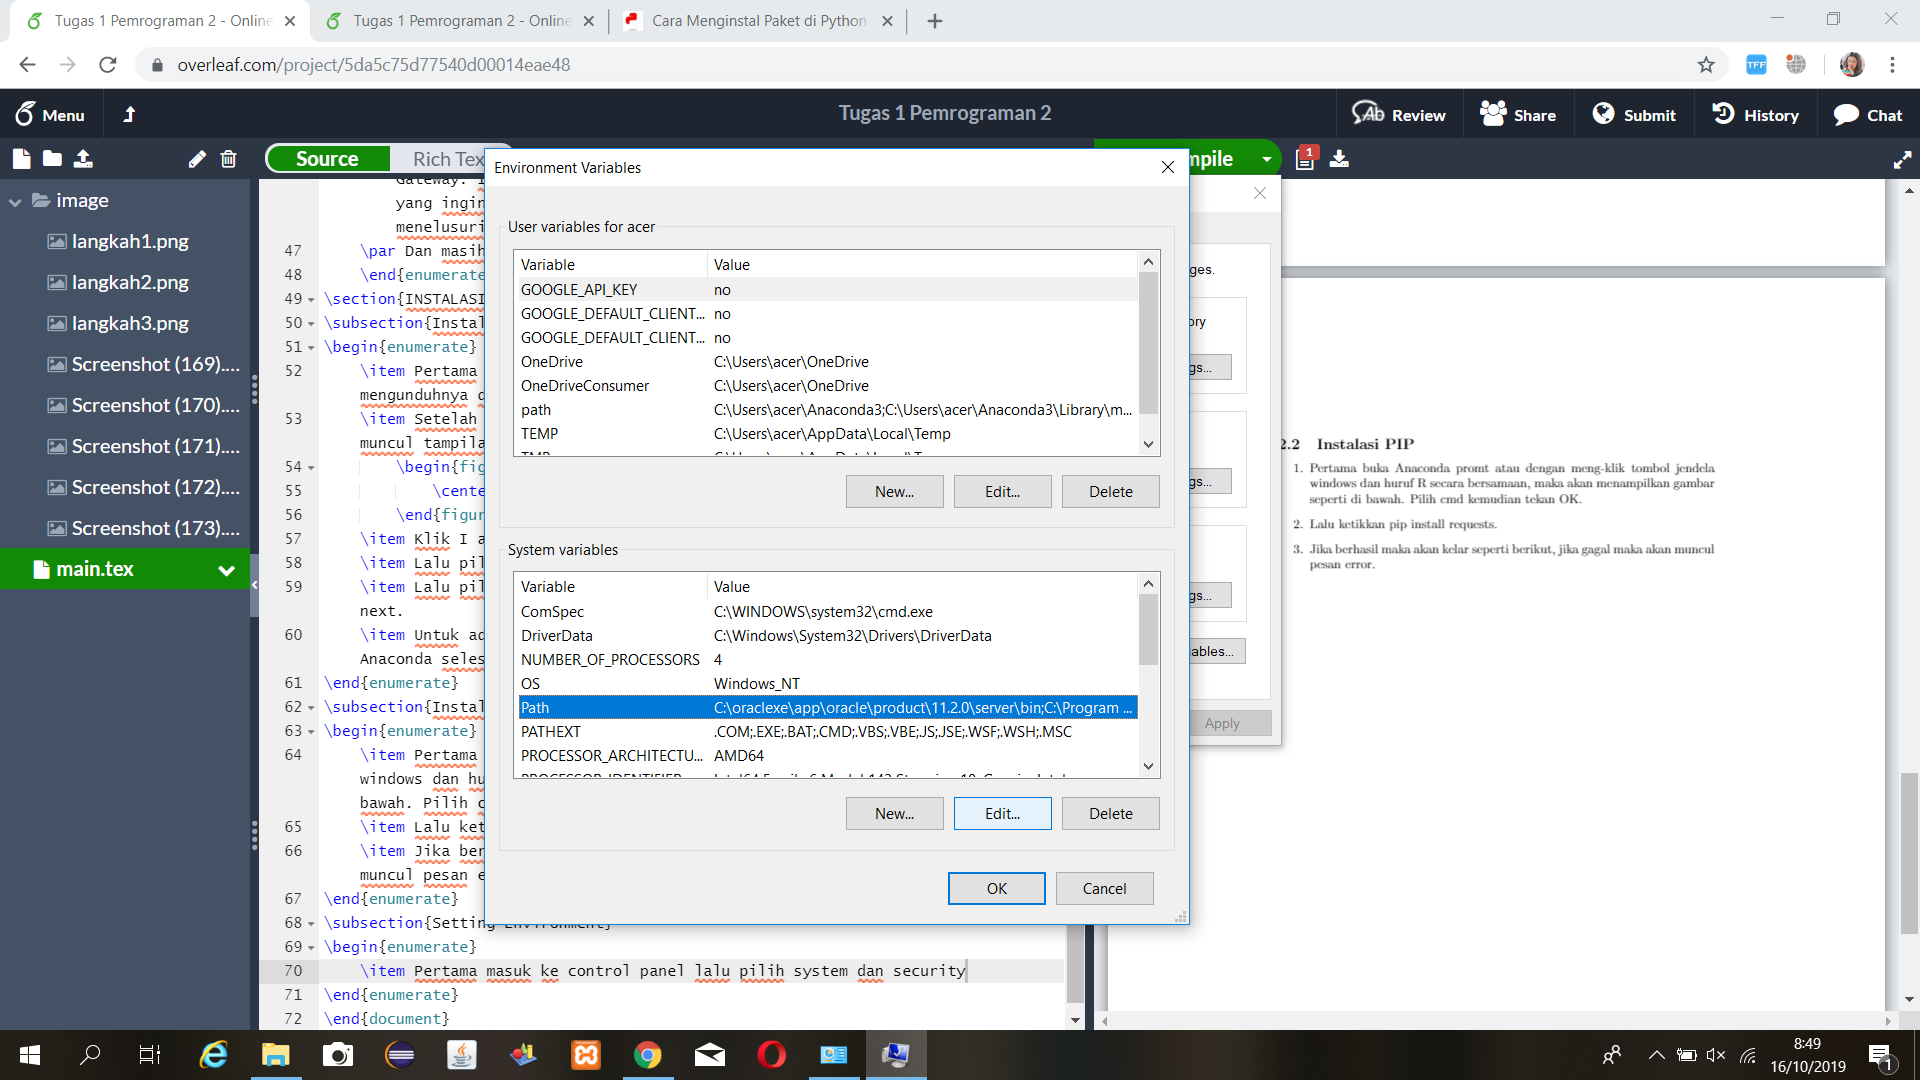
\includegraphics[width=8cm]{image/pathedit.png}}
        \end{figure}
        \paragraph{}
            \centerline{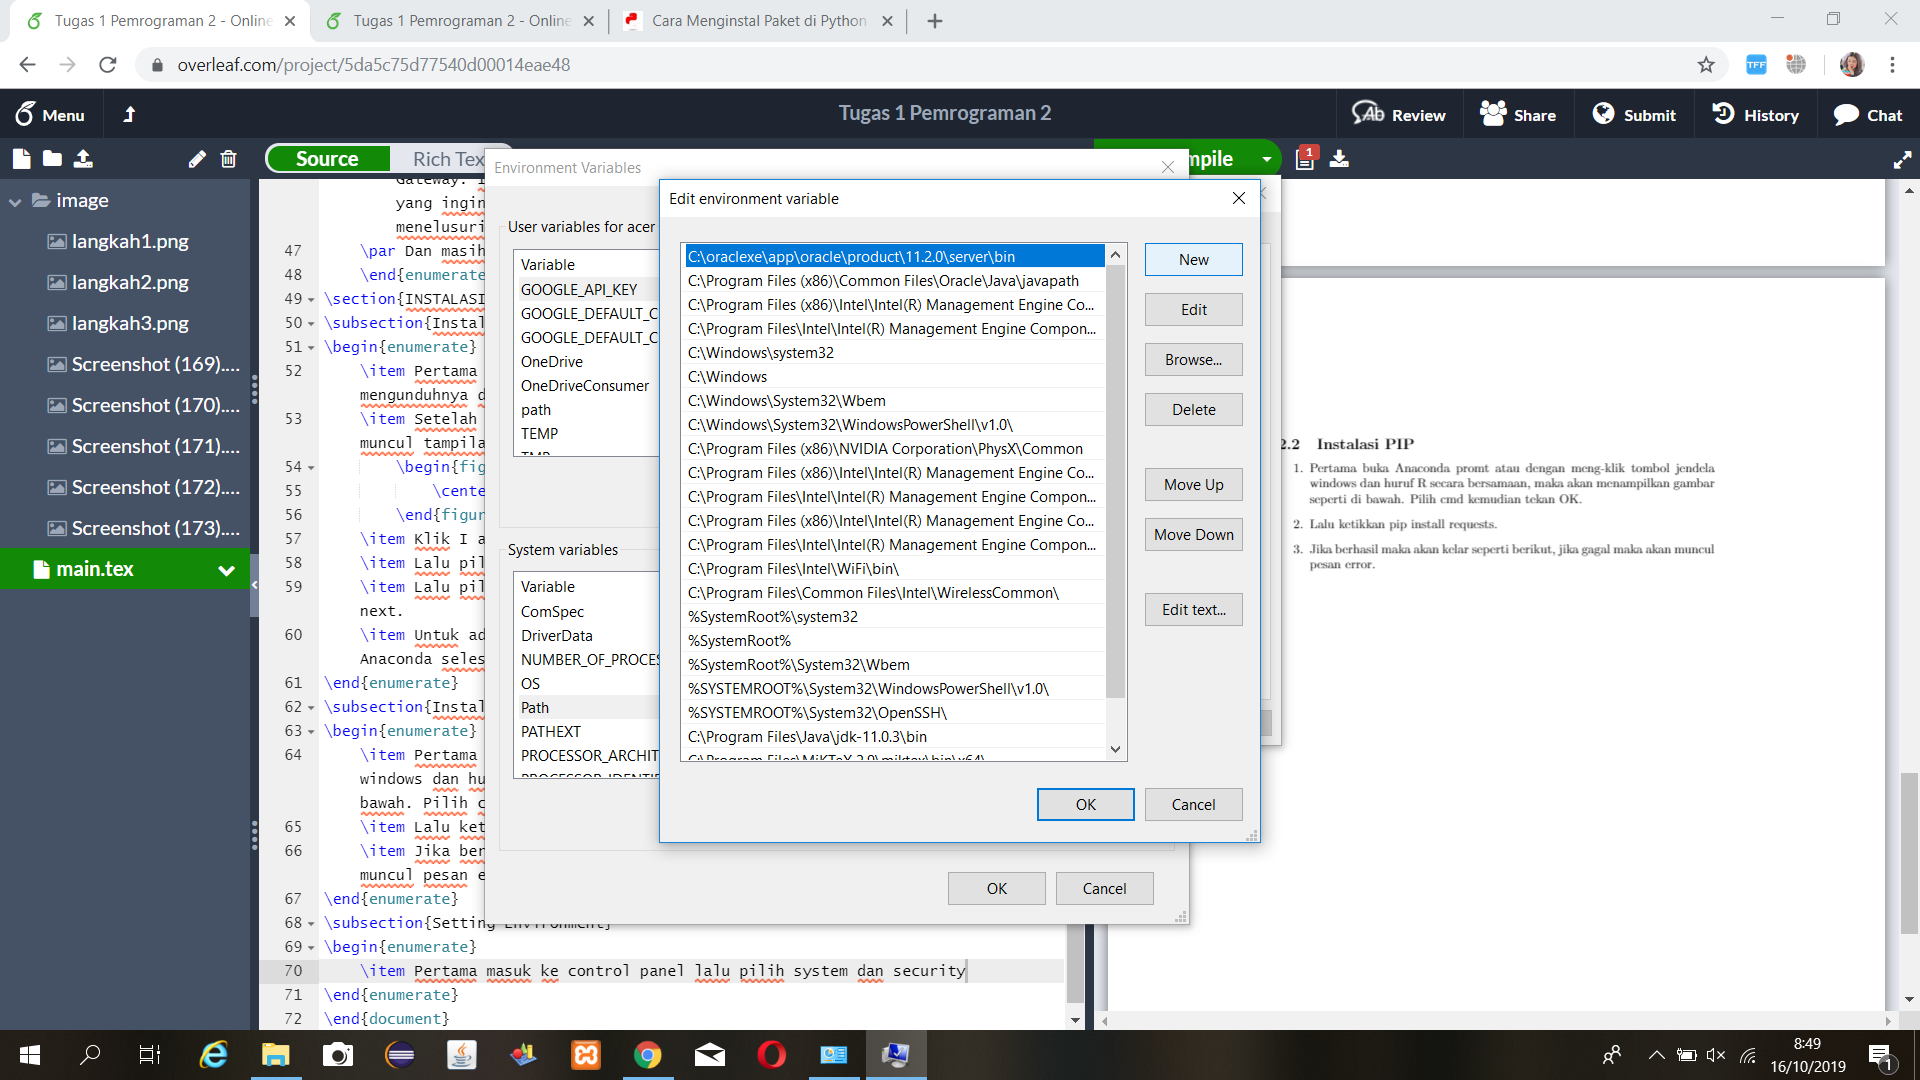
\includegraphics[width=8cm]{image/new.png}}
        \paragraph{}
            \centerline{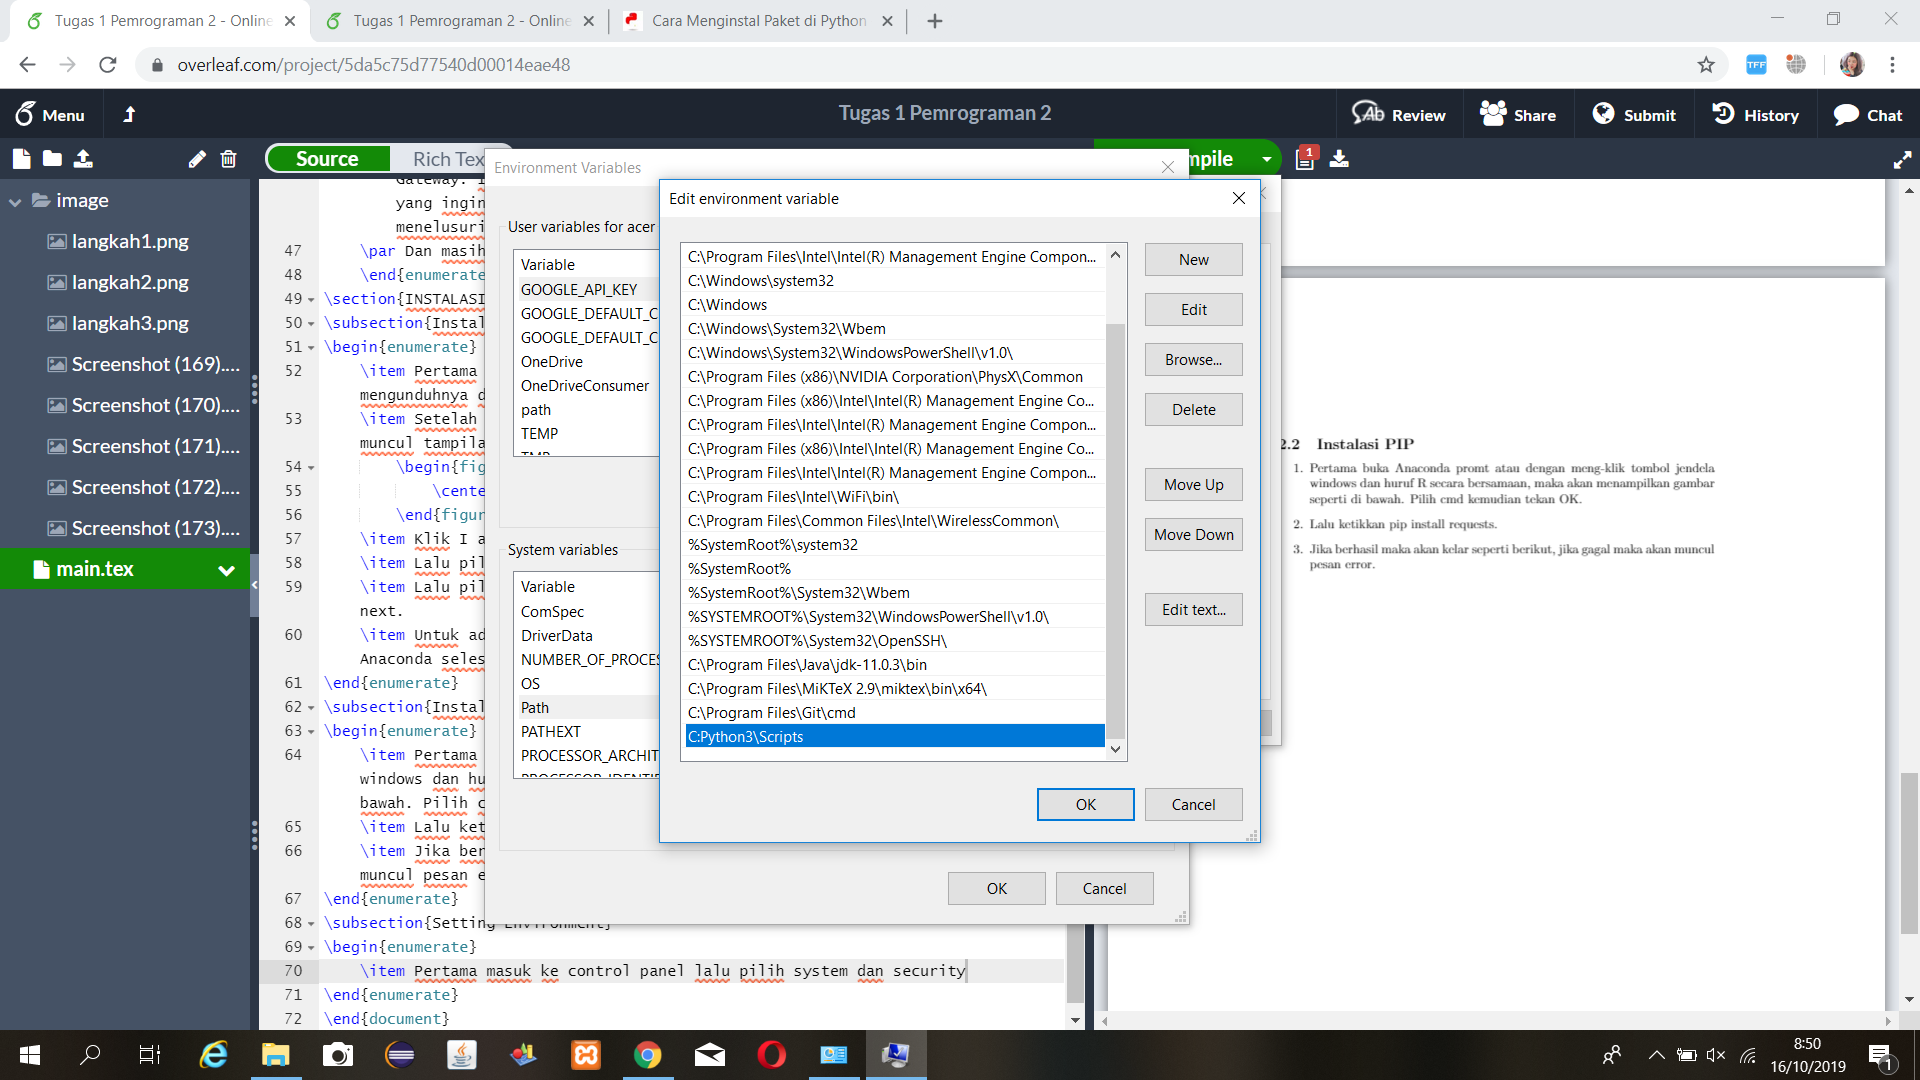
\includegraphics[width=8cm]{image/pathnewok.png}}
\end{enumerate}
\subsection{Mencoba Interpreter/CLI pada CMD}
\begin{enumerate}
    \item Pertama buka Cmd terlebih dahulu pada PC/Laptop anda.
        \begin{figure}[h]
            \centerline{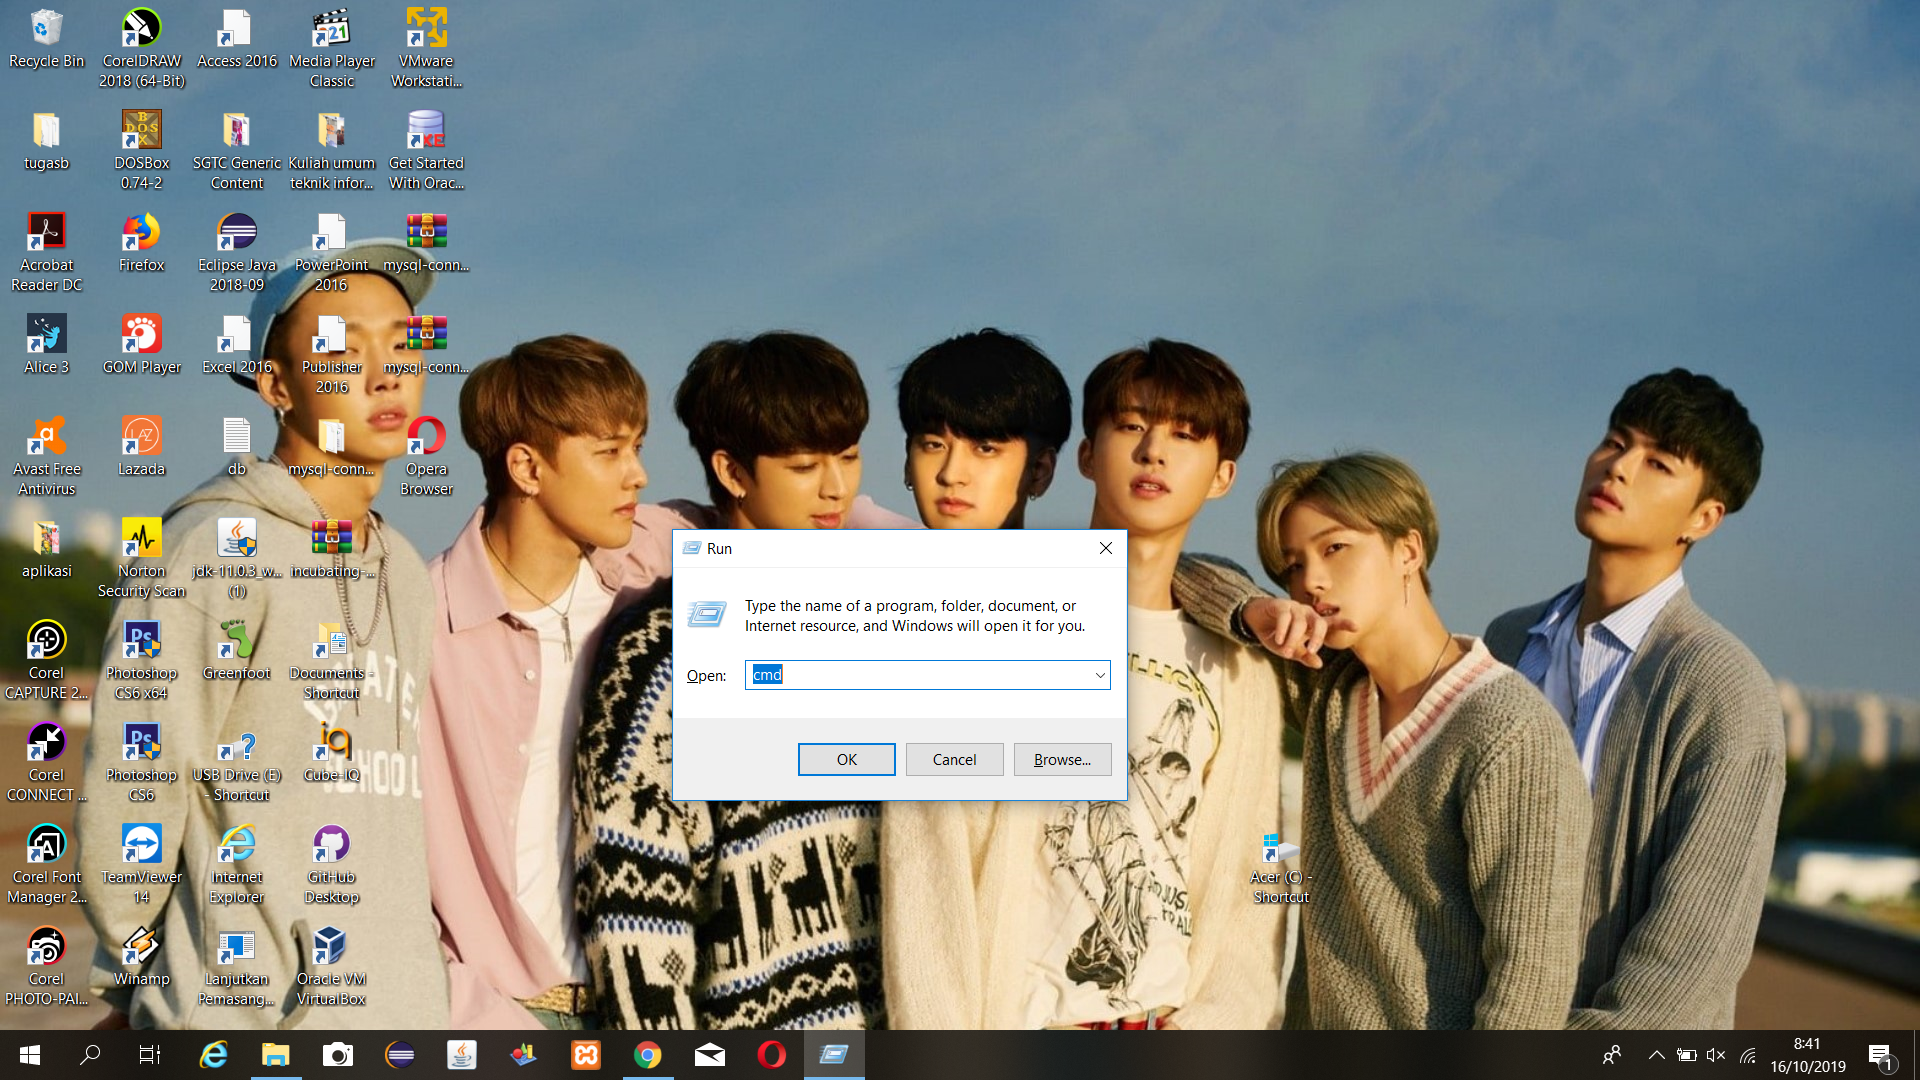
\includegraphics[width=8cm]{image/cmd.png}}
        \end{figure}
    \item Kemudian ketikkan Python
        \begin{figure}[h]
            \centerline{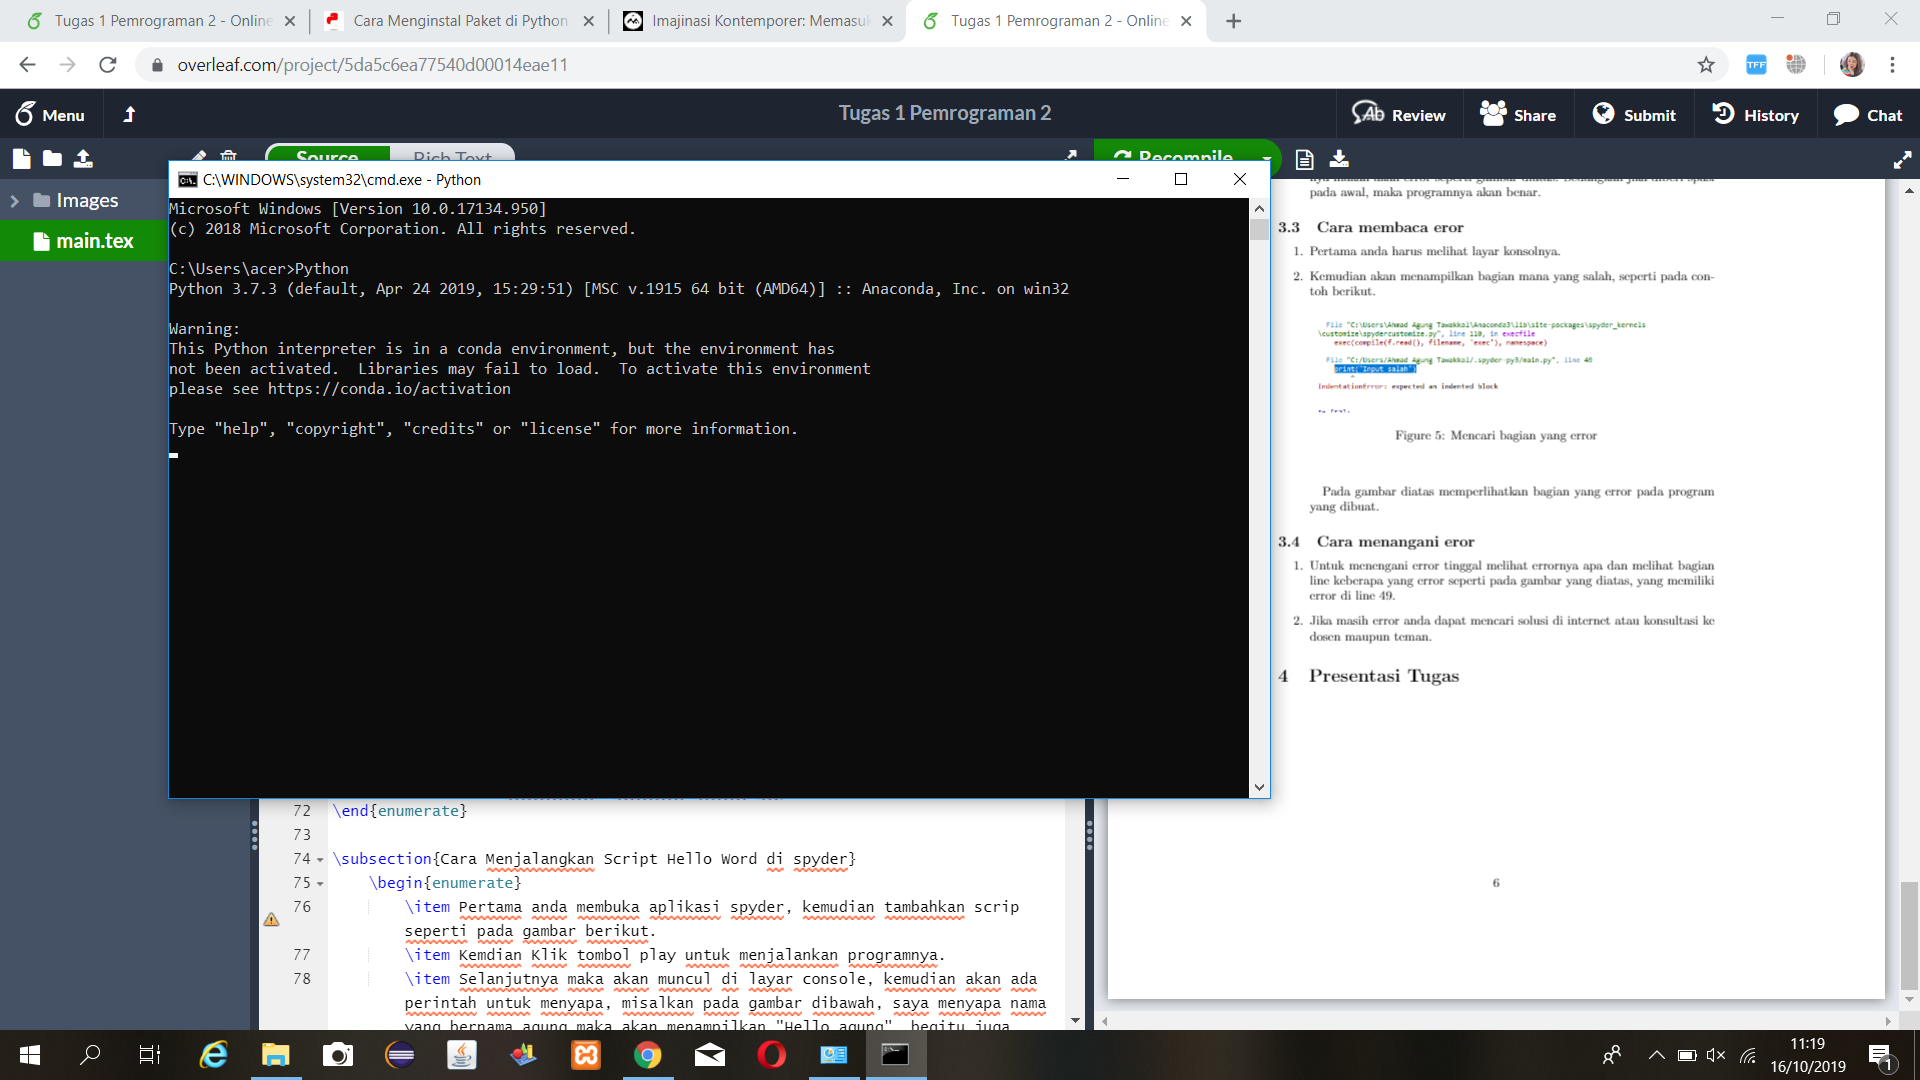
\includegraphics[width=8cm]{image/python.png}}
        \end{figure}
    \item Lalu ketikkan print("Hello World!")
    \paragraph{}
            \centerline{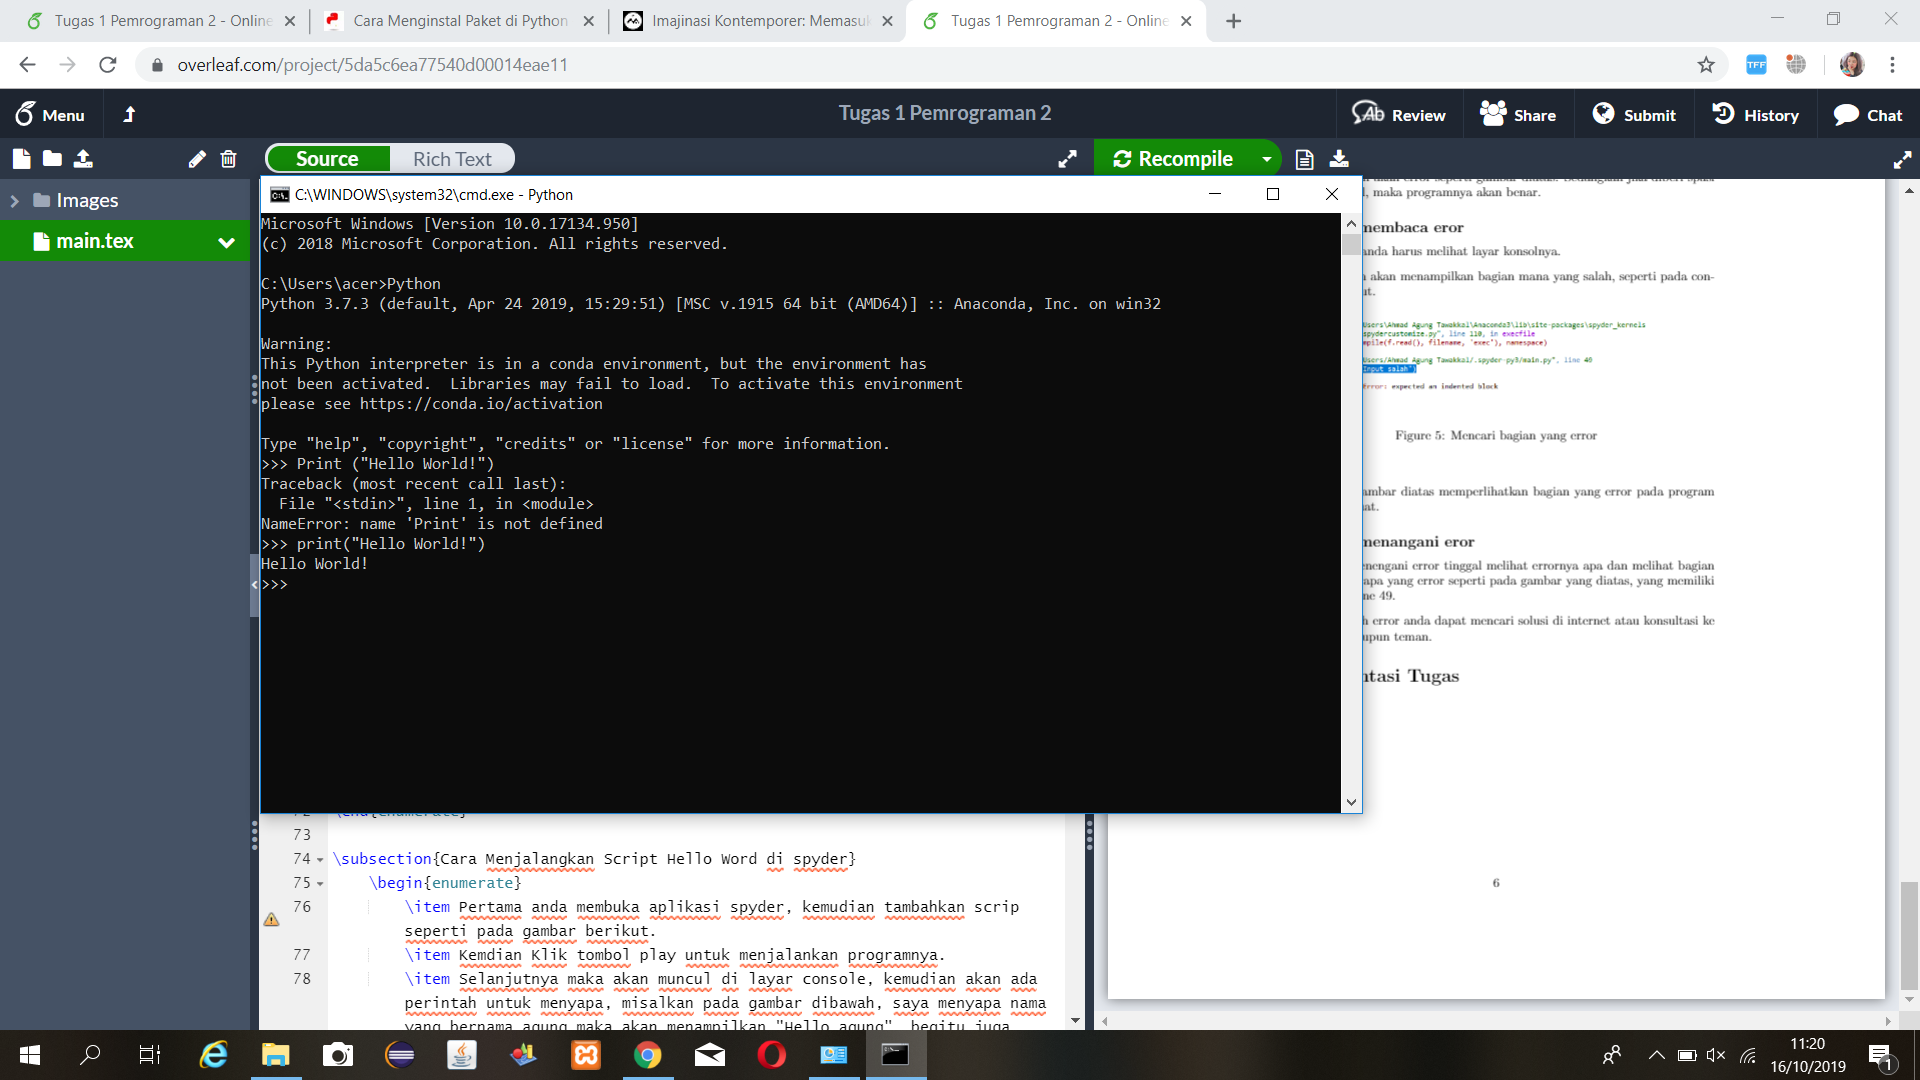
\includegraphics[width=8cm]{image/printhelloworld.png}}
\end{enumerate}
\subsection{Menjalankan dan Mengupdate Anaconda dan Spyder}
\begin{enumerate}
    \item Pertama download terlebih dahulu aplikasi Anaconda
    \item Lalu install
    \item Setelah terinstall buka Anaconda
    \item Di dalamnya terdapat Spyder dan lain lain.
    \item Untuk mengupdate Anaconda, silahkan pergi ke cmd lalu ketikkan Conda install -c anaconda python
        \begin{figure}[h]
            \centerline{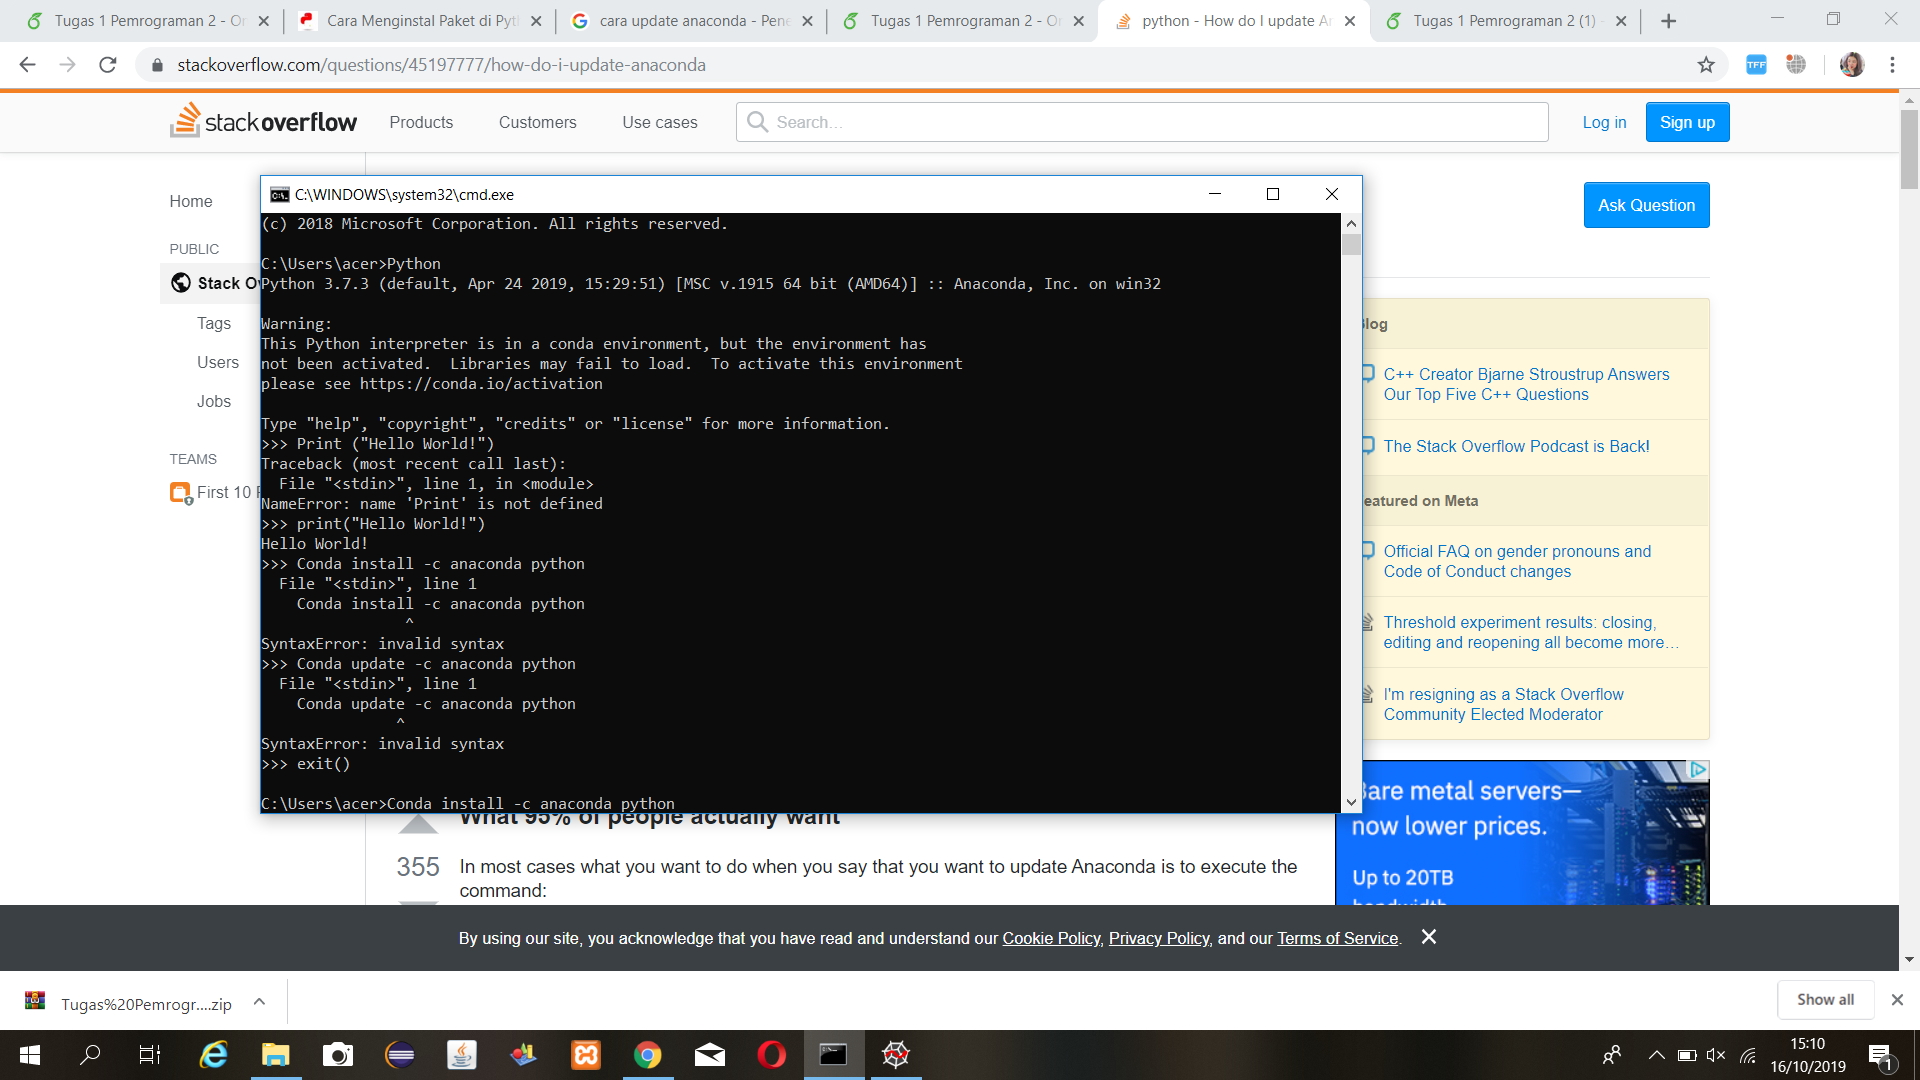
\includegraphics[width=8cm]{image/anacondaupdt.png}}
        \end{figure}
\end{enumerate}
\subsection{Menjalankan Script "Hello World!" di Spyder}
\begin{enumerate}
    \item Pertama buka lah aplikasi Spyder
    \paragraph{}
            \centerline{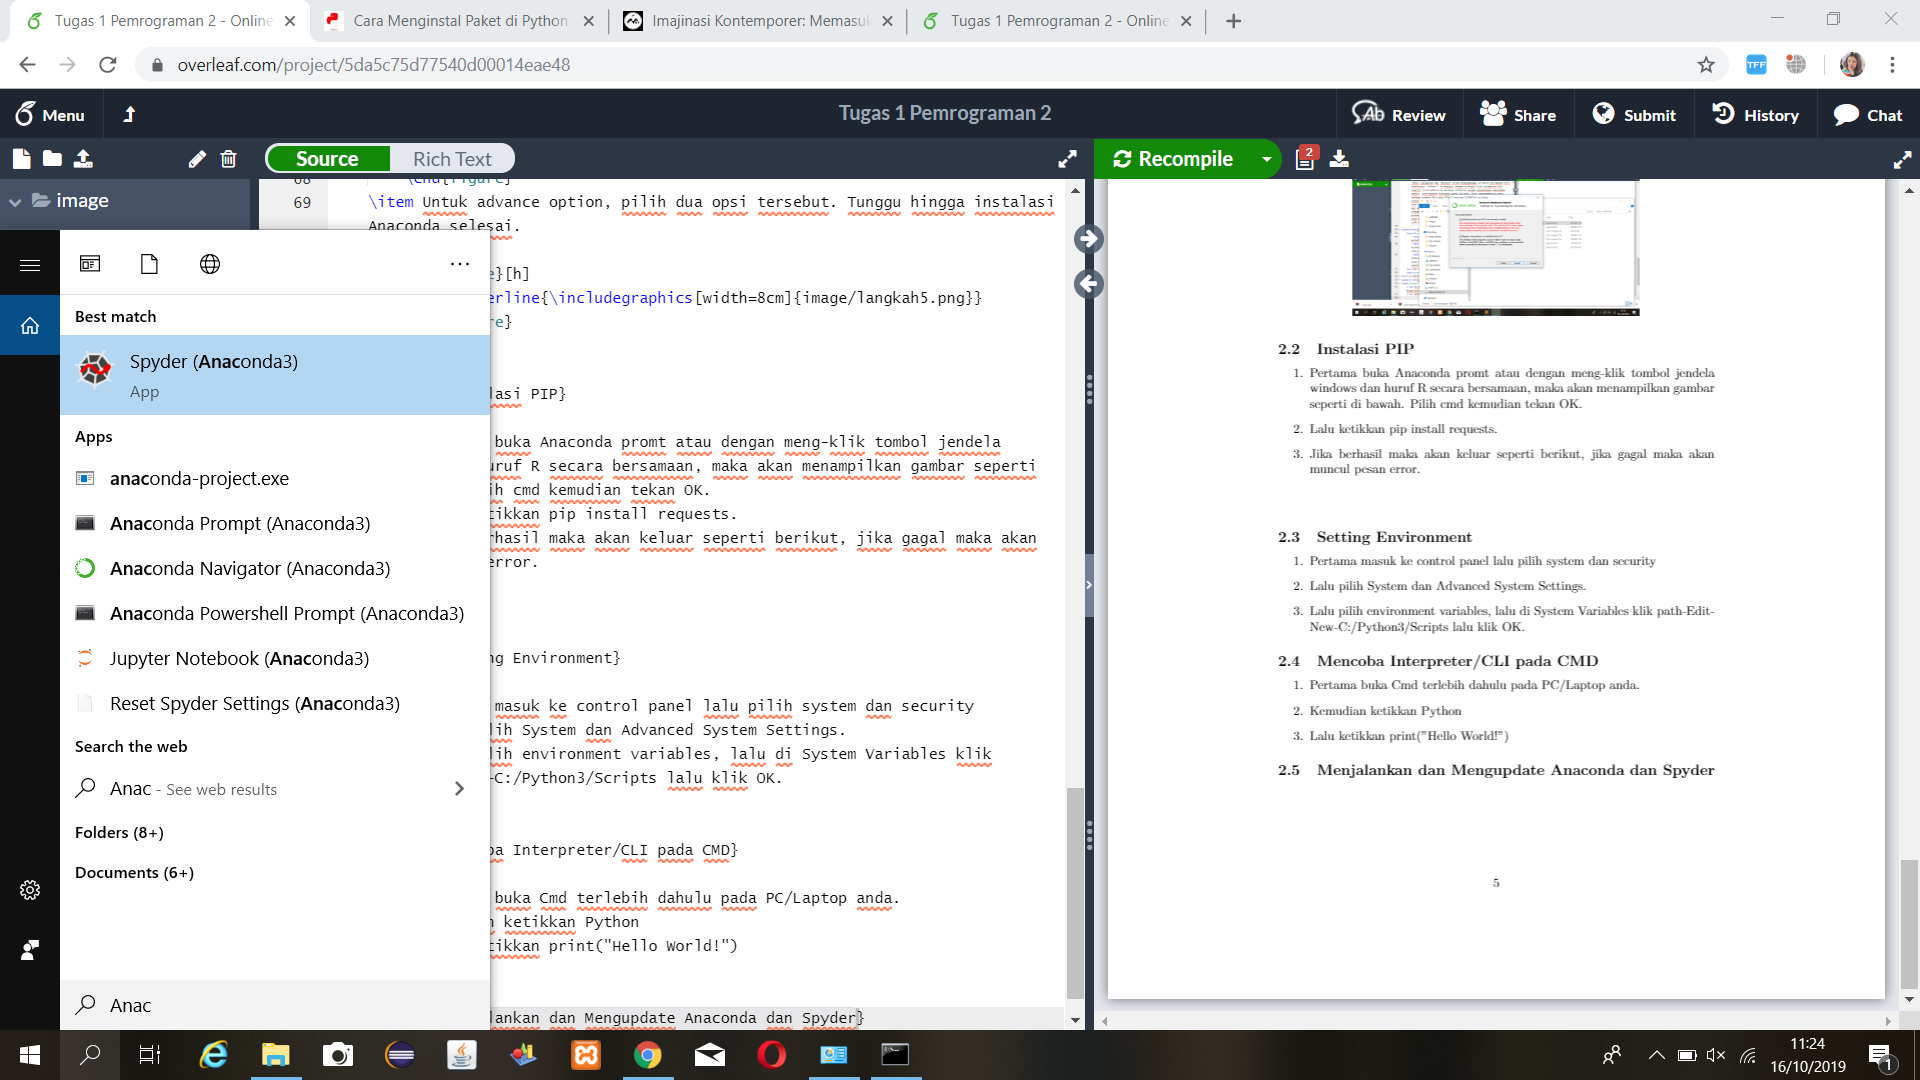
\includegraphics[width=8cm]{image/spyder.png}}
    \item Lalu ketikkan script seperti berikut
        \begin{figure}[h]
            \centerline{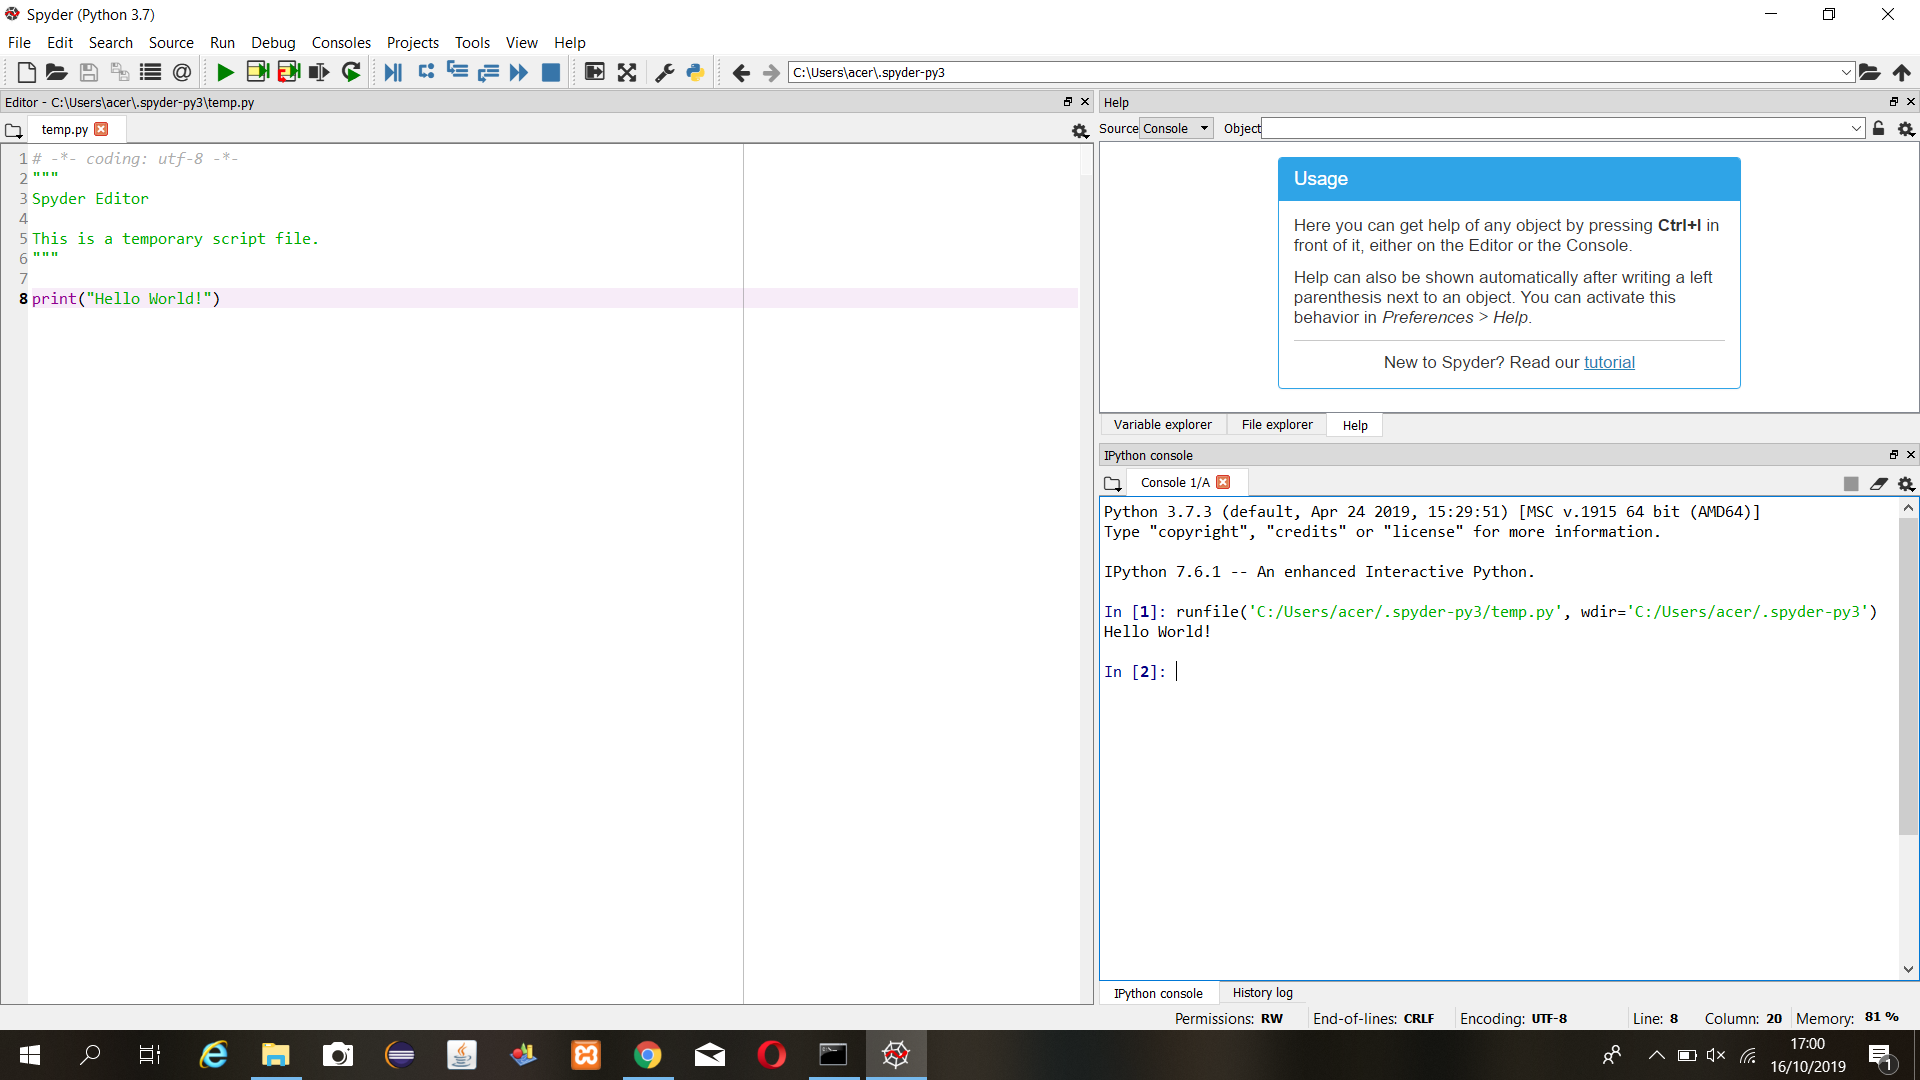
\includegraphics[width=8cm]{image/helloworld.png}}
        \end{figure}
    \item Lalu akan ditampilkan pada console, maka hasilnya "Hello World!"
\end{enumerate}

\subsection{Menjalankan Login Otomatis dengan Library Selenium dan Inputan User}
\begin{enumerate}
    \item Pertama buka cmd terlebih dahulu
    \item Lalu install Selenium dengan cara ketikkan "pip install selenium"
        \paragraph{}
            \centerline{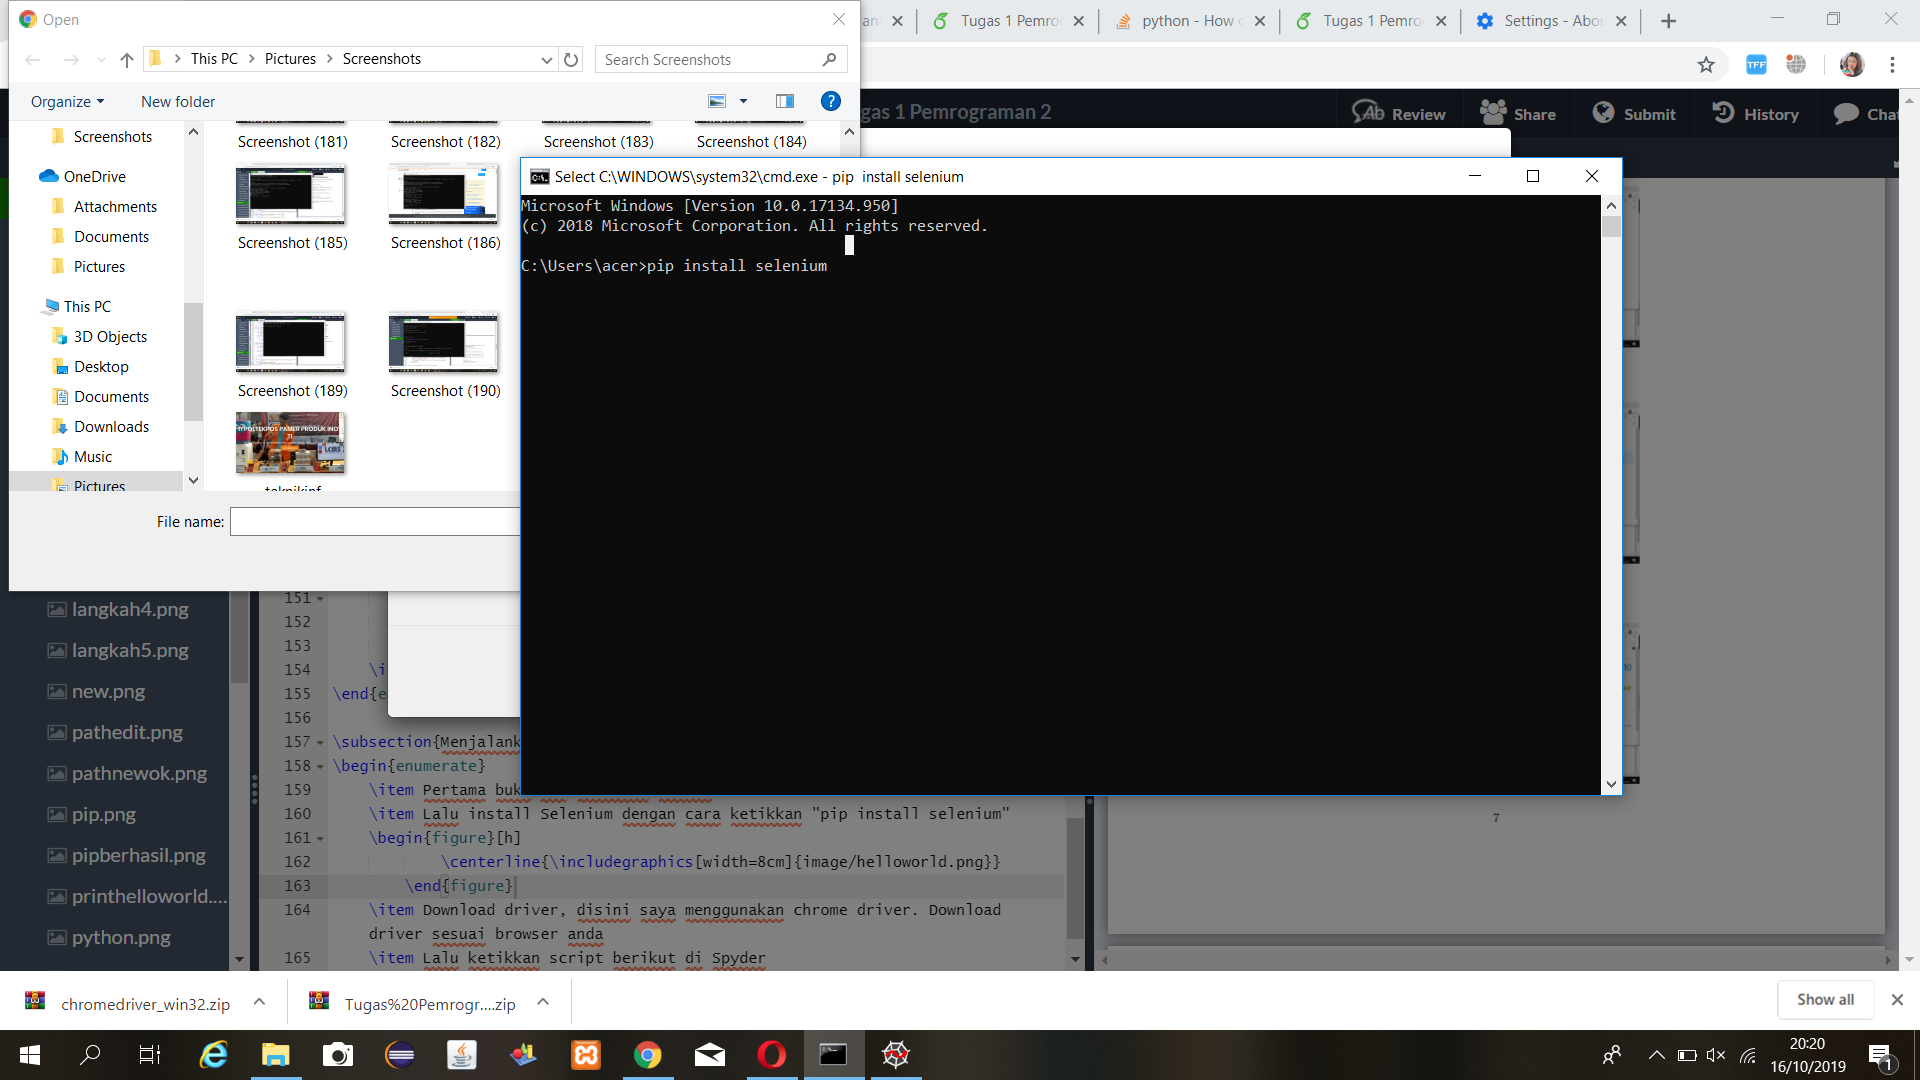
\includegraphics[width=8cm]{image/pipinstallsel.png}}
    \item Download driver, disini saya menggunakan chrome driver. Download driver sesuai browser anda
        \begin{figure}[h]
            \centerline{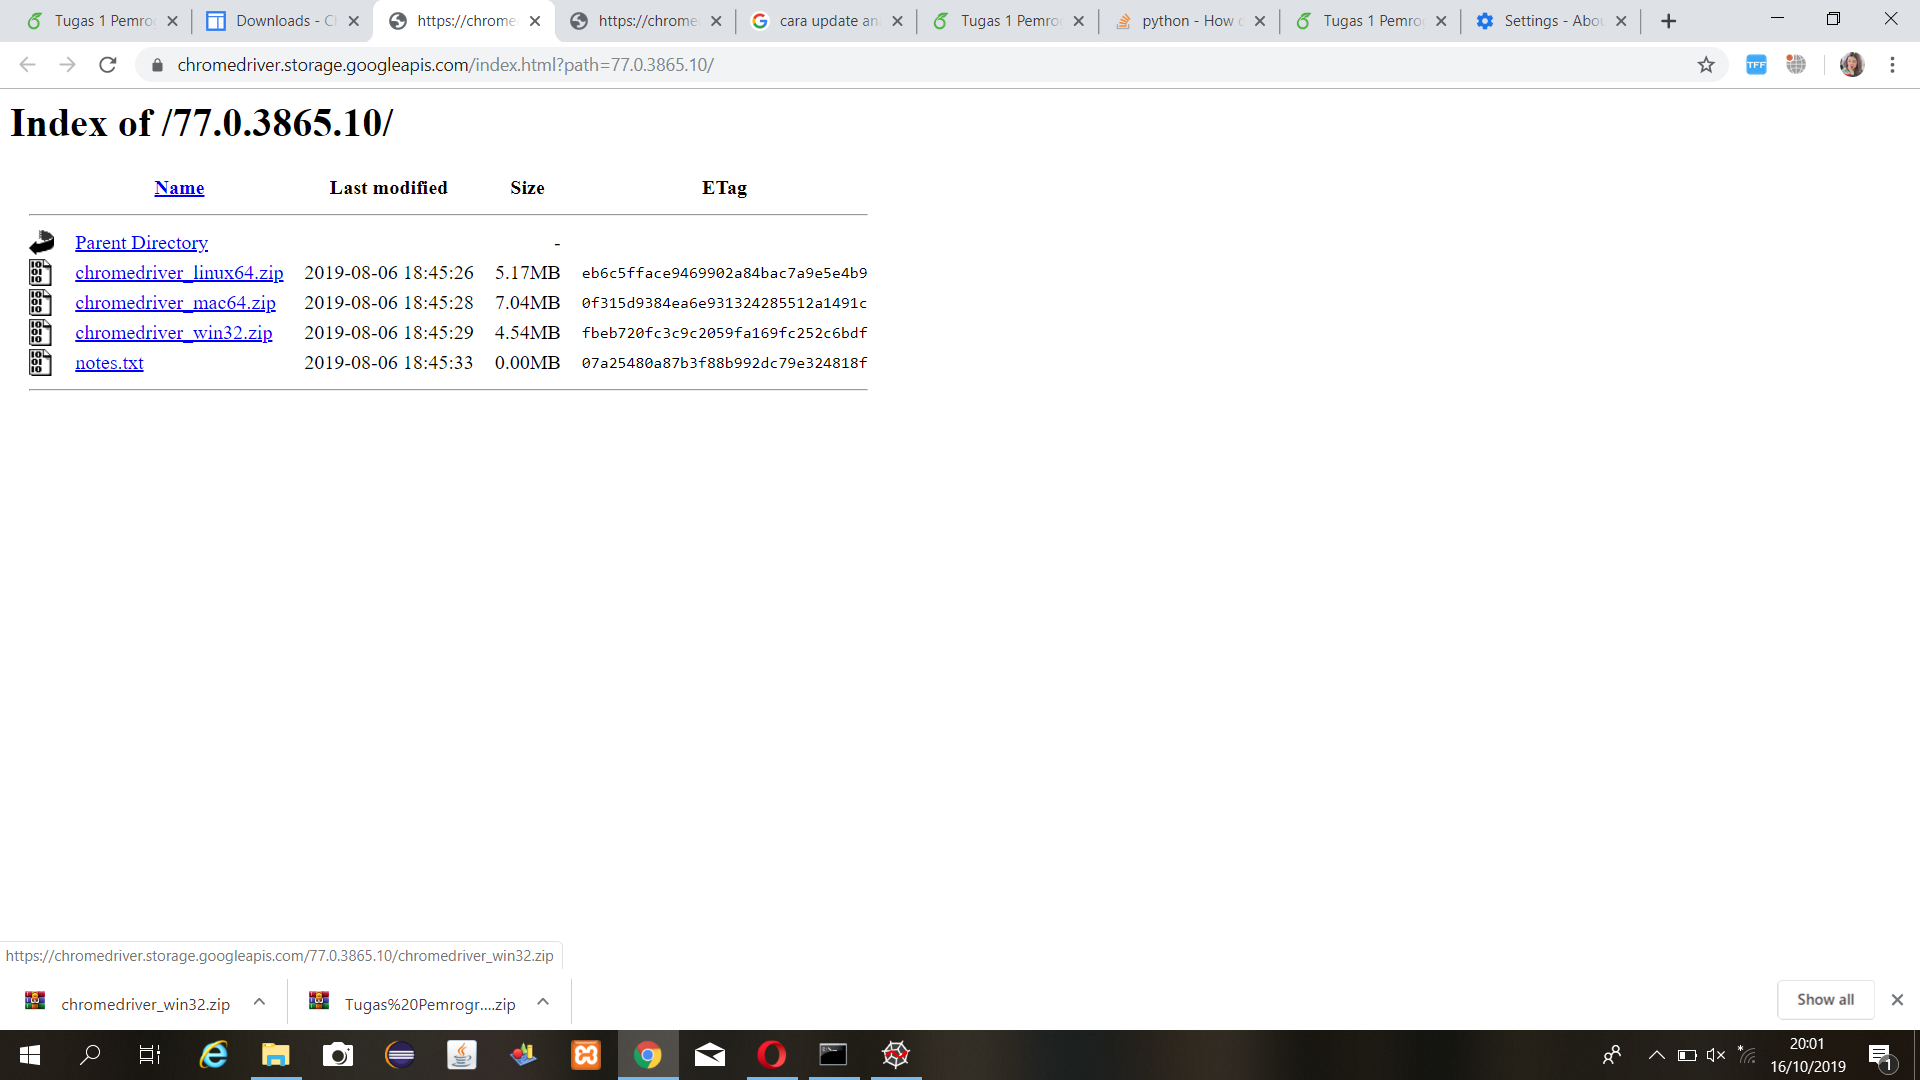
\includegraphics[width=8cm]{image/chromedriver.png}}
        \end{figure}
    \item Lalu ketikkan script berikut di Spyder
        \begin{figure}[h]
            \centerline{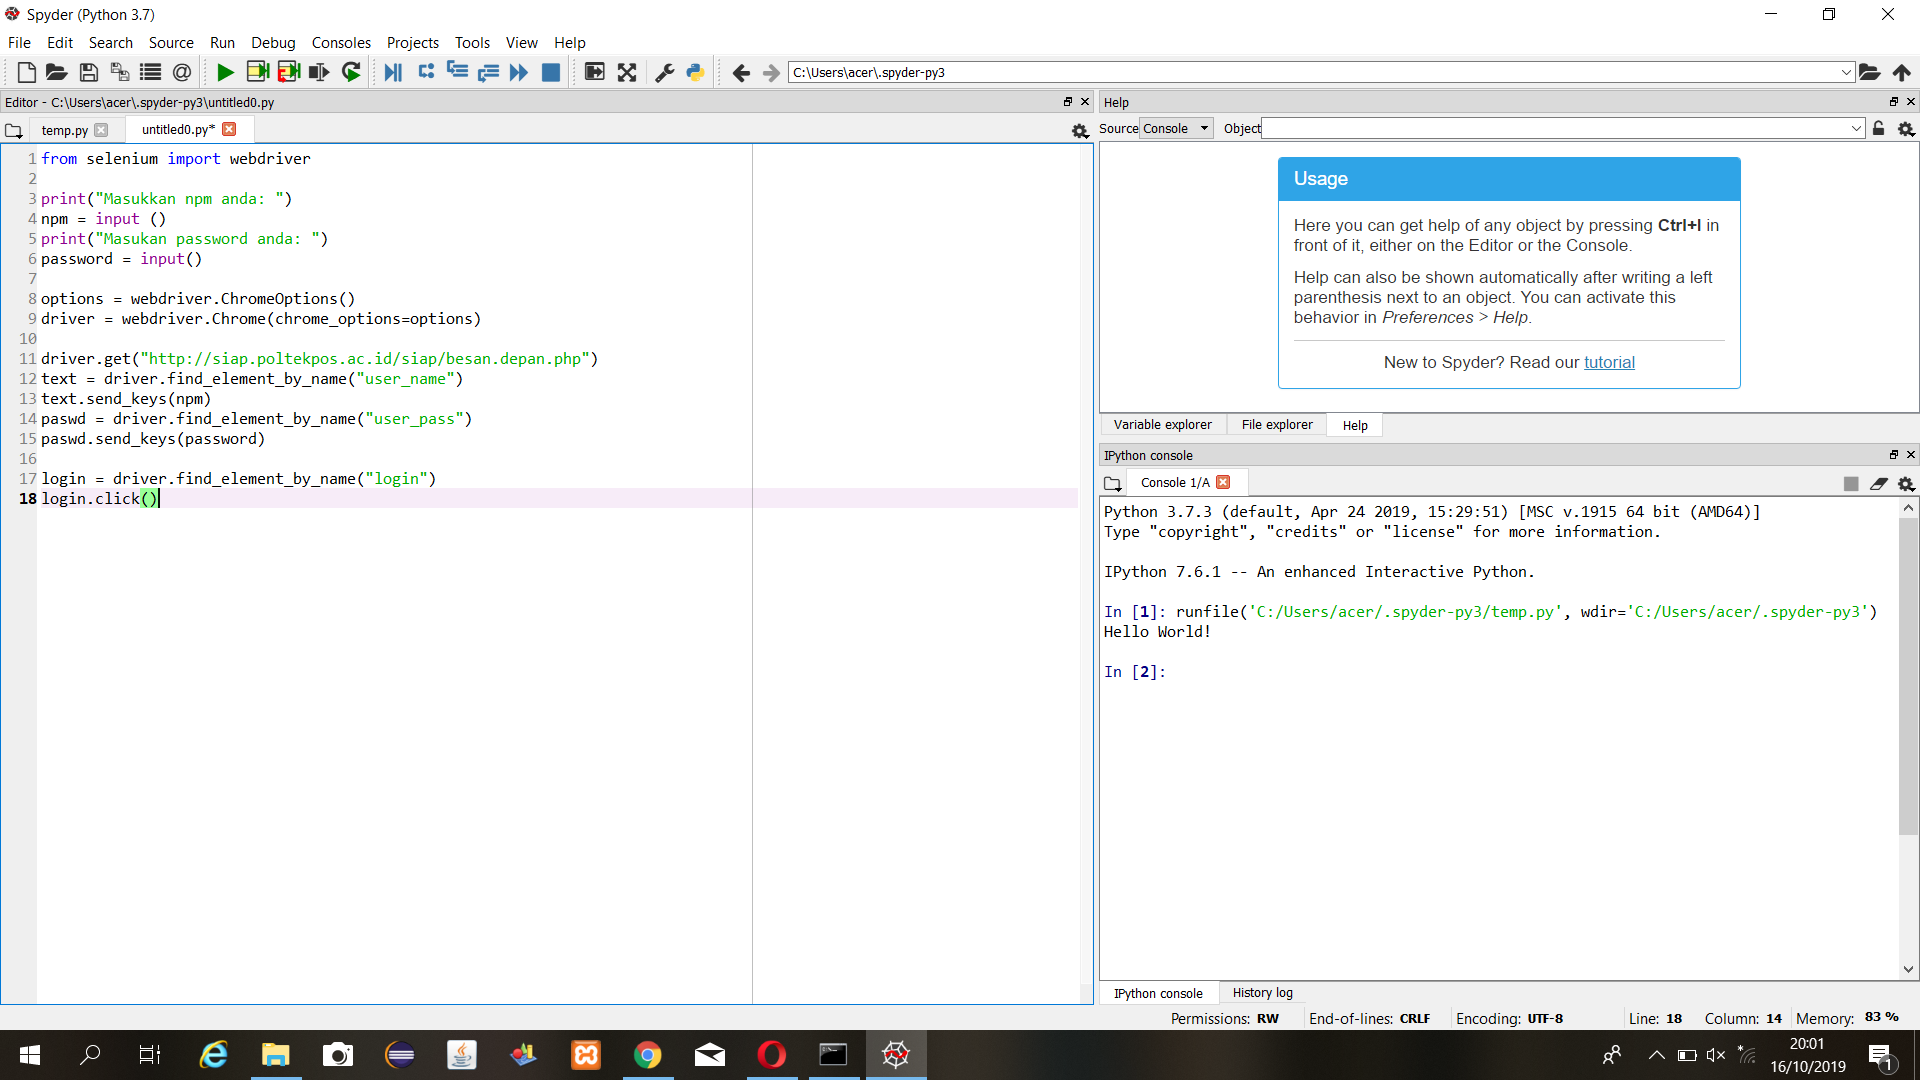
\includegraphics[width=8cm]{image/scriptsele.png}}
        \end{figure}
    \item Lalu run, setelah itu akan login otomatis ke browser yang anda tuju
\end{enumerate}

\subsection{Cara Menggunakan Variabel Explorer pada Spyder}
\begin{enumerate}
    \item Buka aplikasi Spyder pada PC/laptop anda
    \item Pada program anda, tambahkan variabel a yang bertipe integer nilai nya bebas, begitu pula dengan variabel b
    \item Variabel c merupakan hasil dari penjumlahan variabel a dan b, c = a+b
    \item Hasilnya akan diperlihatkan dengan jelas pada variabel explore
        \begin{figure}[h]
            \centerline{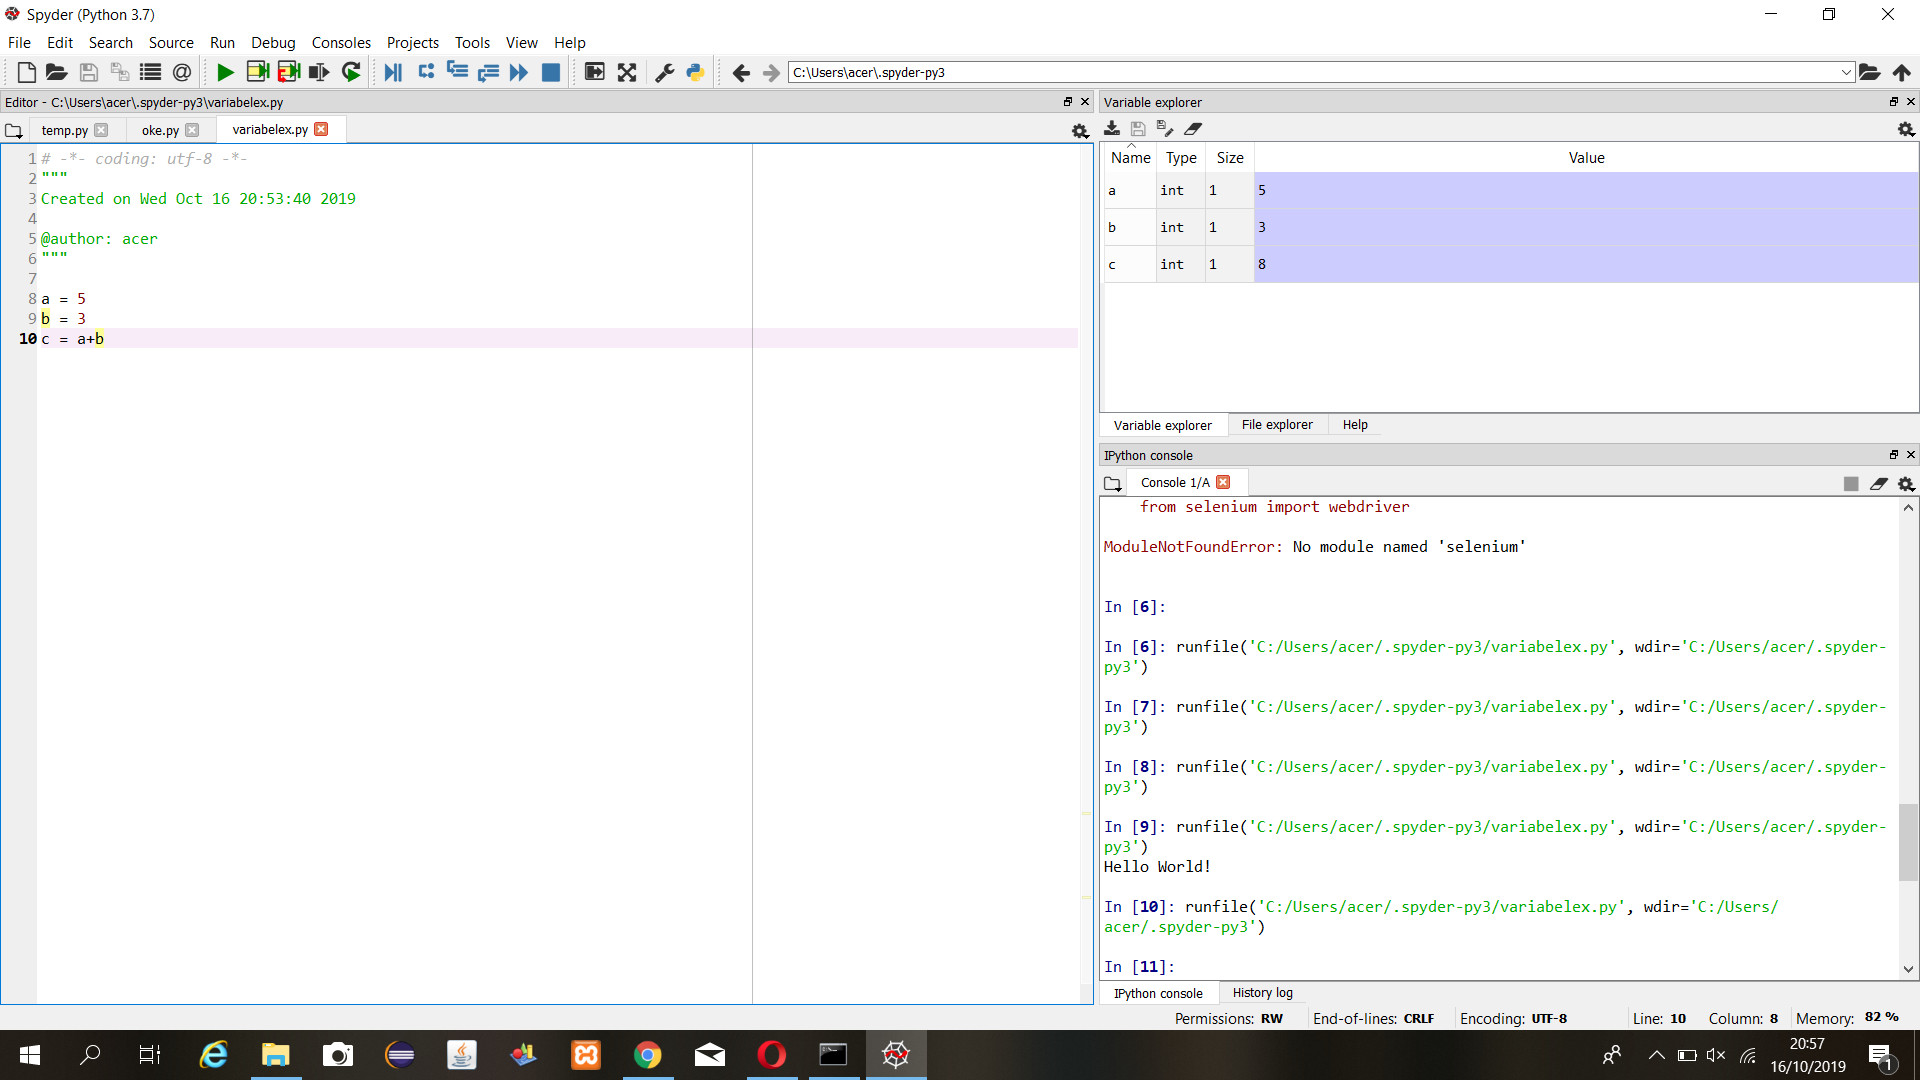
\includegraphics[width=8cm]{image/variabelex.png}}
        \end{figure}
\end{enumerate}

\section{Identasi}
\subsection{Pengertian Identasi}
\paragraph{}
    Identasi adalah bagian awal paragraf yang menjorok ke dalam pada setiap baris paragraf.
\subsection{Jenis-Jenis Error Identasi yang Ditemukan}
\begin{enumerate}
    \item Identasi If
    \item Identasi Else
    \item Identasi Elif
\end{enumerate}
\subsection{Contoh Error dan Benar}
\begin{enumerate}
    \item Contoh Error
    \paragraph{}
        \centerline{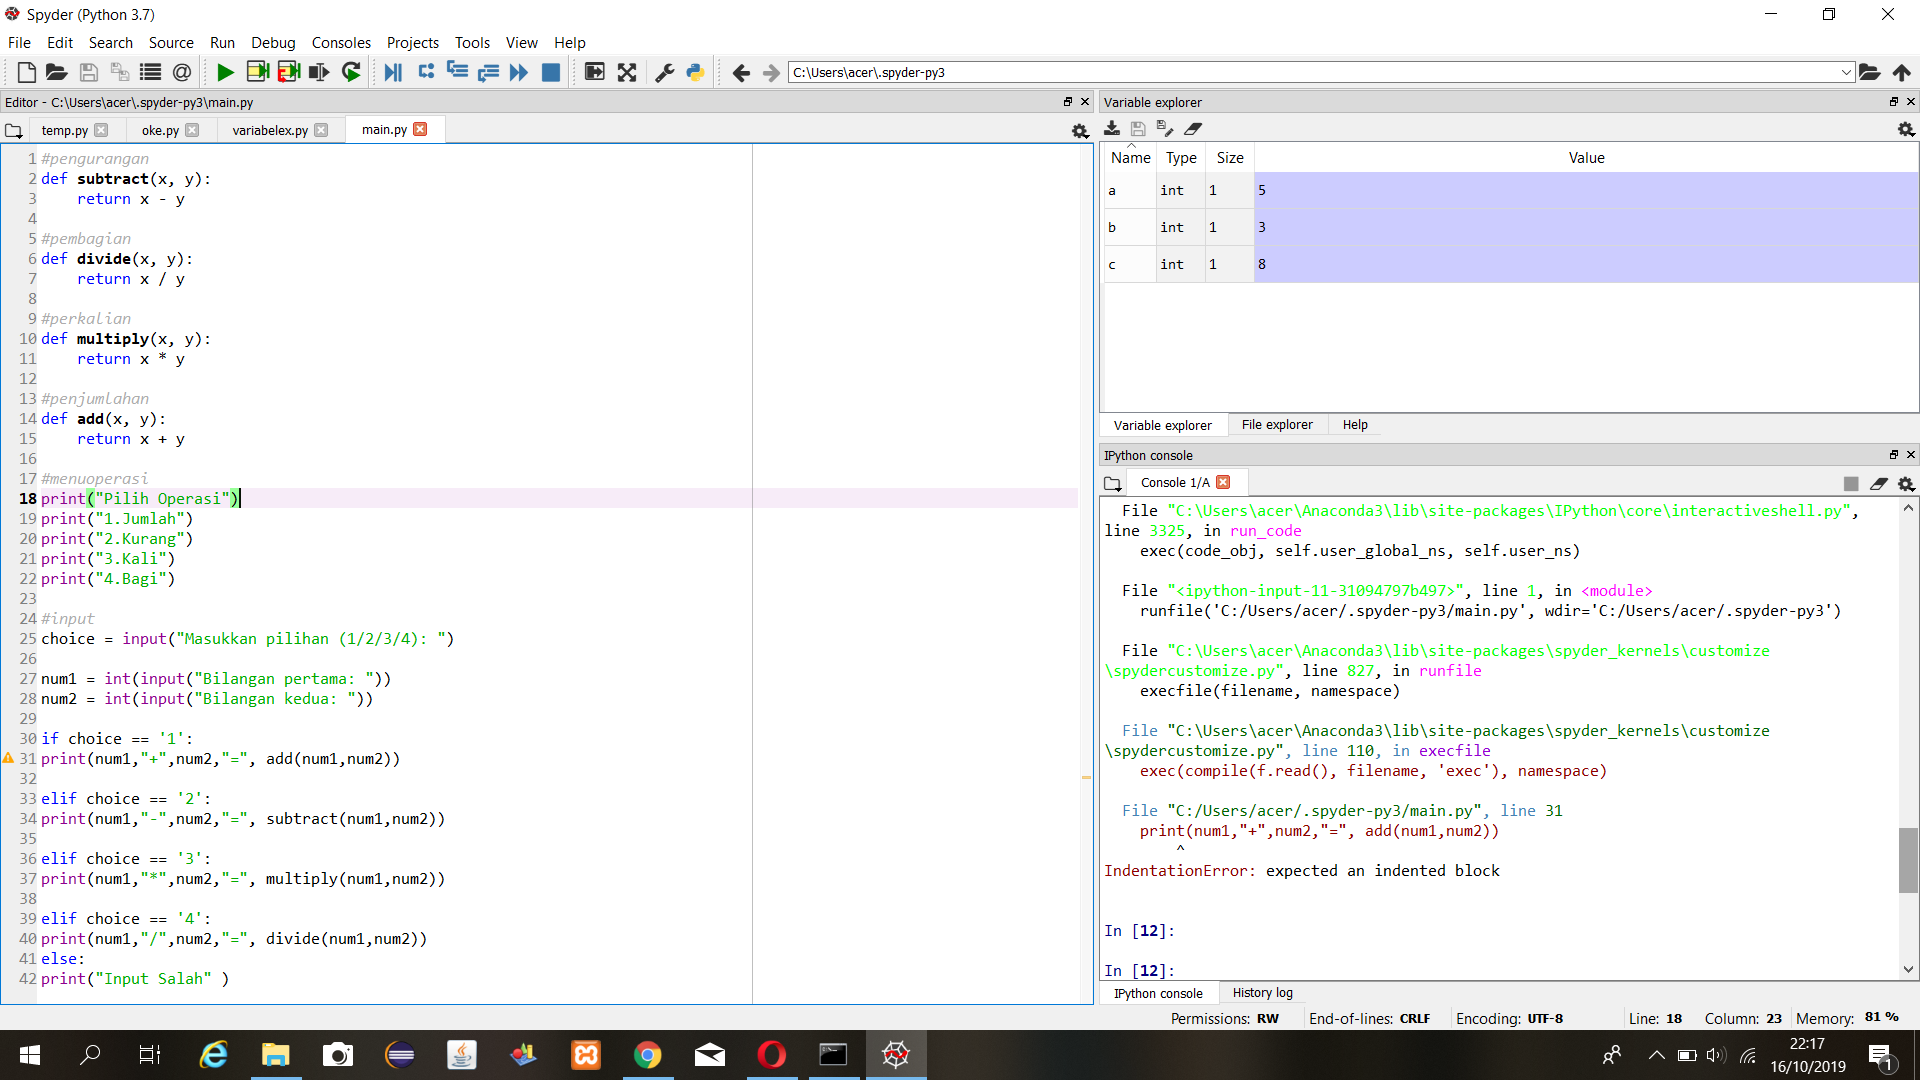
\includegraphics[width=8cm]{image/error.png}}
    \item Contoh Benar
    \begin{figure}[h]
            \centerline{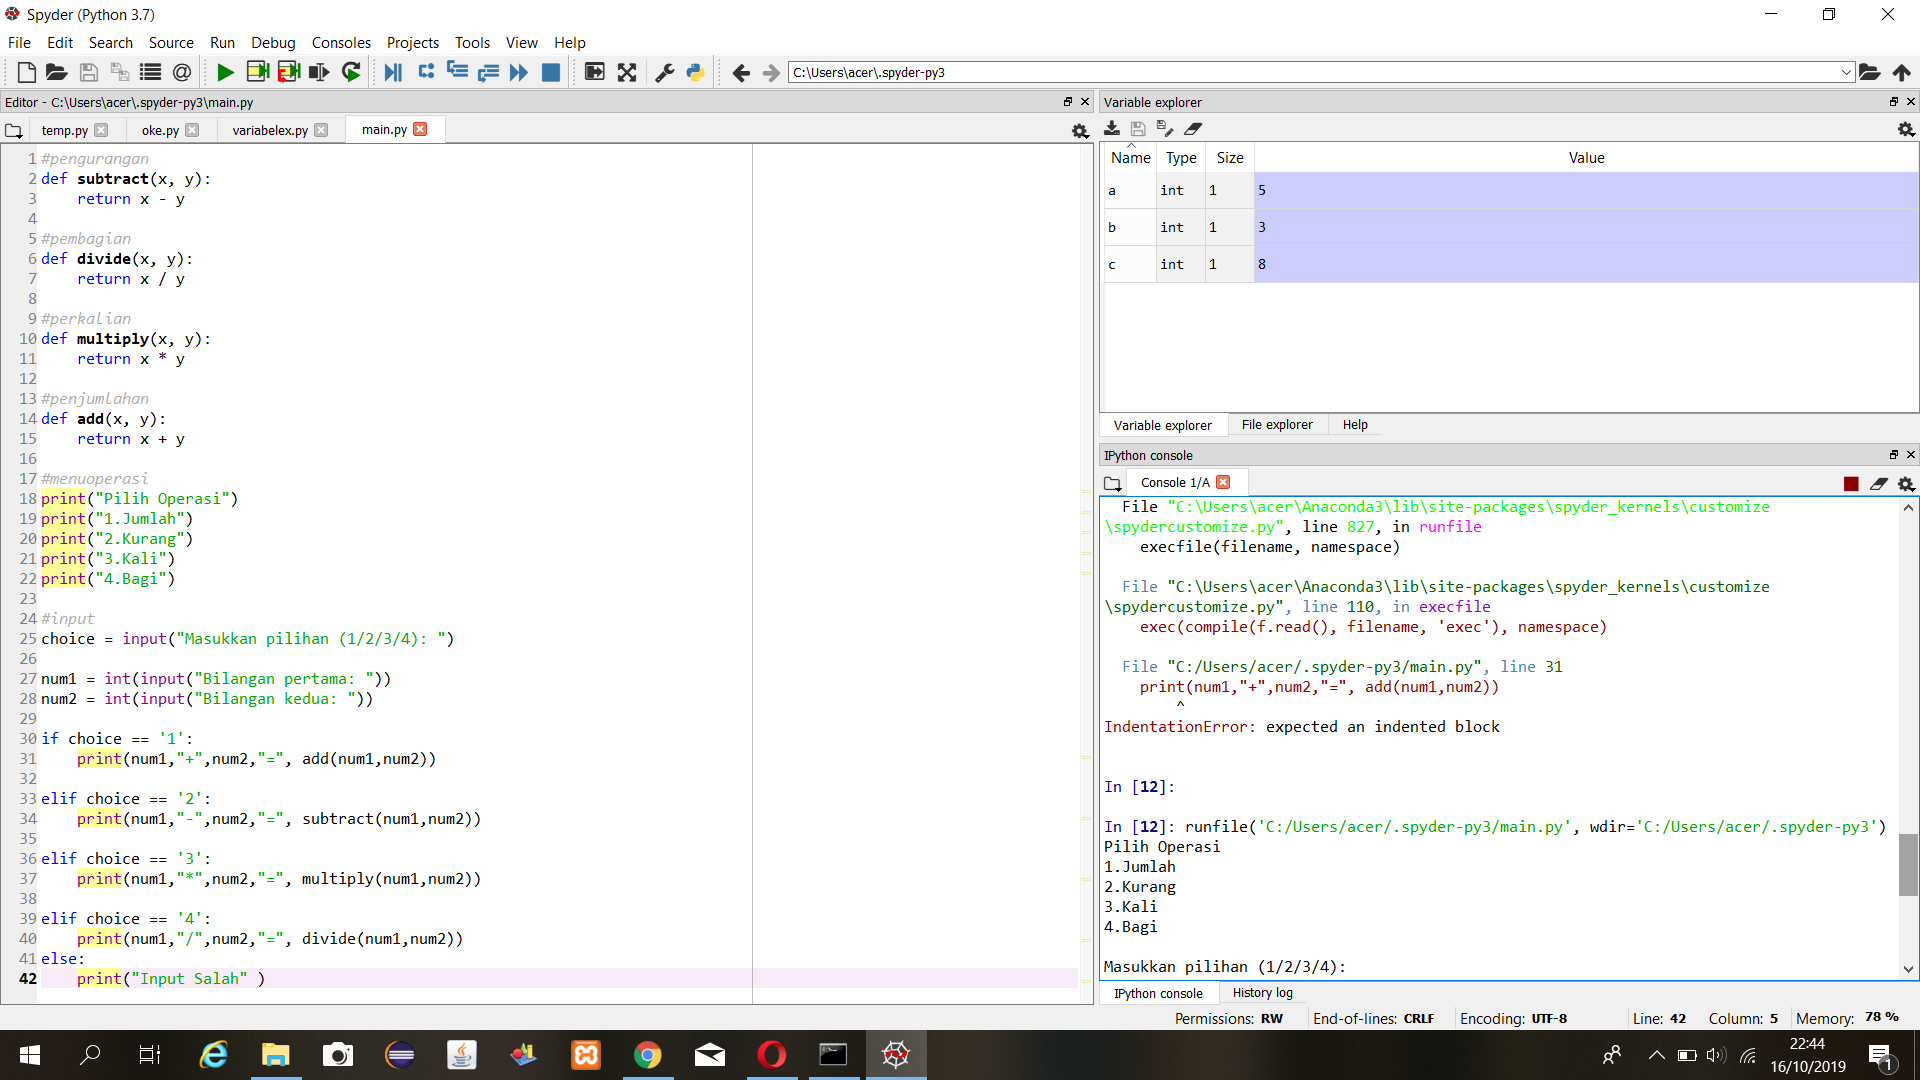
\includegraphics[width=8cm]{image/contohbenar.png}}
        \end{figure}
\end{enumerate}
\end{document}
